\documentclass{SPhdThesis}
\usepackage{siunitx}
\usepackage{placeins}
\usepackage{xspace}
\usepackage{xstring}
\usepackage{xfrac}
\usepackage{appendix}
\usepackage{ccaption}

\usepackage[backend=bibtex, style=authoryear, maxbibnames=3, maxcitenames=1, backref=true]{biblatex}
	
\addbibresource{biblio.bib}
\hypersetup{plainpages=false, colorlinks=true, linkcolor={black}, citecolor={webblue}, urlcolor=webblue} % Colors hyperlinks in blue - change to black if annoying
\DefineBibliographyStrings{english}{%
  backrefpage = {page},% originally "cited on page"
  backrefpages = {pages},% originally "cited on pages"
}


% PDF and title properties.
\SgSetTitle{Interaction dynamics of cytoskeletal polymers}
\SgSetAuthor{Jochen Krattenmacher}
\SgSetAuthorDegrees{Ms. Science}
\SgSetYear{2024}
\SgSetDegree{Doctor of Philosophy}
\SgSetDepartment{Department of Physical and Macromolecular Chemistry}
\SgSetUniversity{Charles University in Prague}


% The document.
\begin{document}
	\begin{frontmatter}
		\SgAddTitle%
            \SgAddDeclaration
		\chapter*{Acknowledgements}
Zdenek
Marcus
Valerie
Manuel and Francois
Alexander
Ilia, Janci
Amayra and Lenka
Whole lab
Imaging facility
Other coauthors
%
		\begin{abstract}
However, the underlying molecular mechanism of how tau as an intrinsically disordered protein can fulfill such regulative functions is still unknown. Here we study how the collective behaviour of tau can influence the activity of motors and severing proteins on microtubules. Using in vitro reconstitution assays, we found that on the microtubule surface tau can form cohesive islands in a pool of diffusible tau molecules. We observed that the islands prevented the interaction of katanin and kinesin-1 motors with the microtubule surface. In contrast, super-processive kinesin-8 motors, which, like katanin and kinesin-1 were able to bind to and move in the regions on the microtubule surface occupied by diffusible tau molecules, additionally, could penetrate the islands where they caused island disassembly. Our results show that two kinetically distinct phases of tau, consisting, respectively, of cooperatively and discretely binding molecules, co-exist on microtubules and differentially regulate the interactions of MAPs with the microtubule surface.
\end{abstract}%
		\SgAddToc%  Table of contents.
		\SgAddLof%  List of figures.
		\SgAddLot%  List of tables.
		\SgAddLoa%  List of algorithms.
	\end{frontmatter}
   
	\chapter{Background}
The biologist Carl Woese suggested that “Organisms are resilient patterns in a turbulent flow—patterns in an energy flow” \parencite{Woese}. If this somewhat captures life, then the formation and maintenance of patterns are essential. On the sub-cellular level, an important component conferring structure and organization is the cytoskeleton. The cytoskeleton is a complex, dynamic network of protein filaments which can be found in the cytoplasm of all cells, including bacteria and archaea. Eukaryotes employ three different types of filaments: microtubules, actin filaments and intermediate filaments. These filaments interact interact with a plethora of other biopolymers in the cell, allowing the cytoskeleton to fulfill vital functions in a diverse set of domains, such as locomotion of the cell, maintaining structural integrity, chromosome segregation and cytokinesis during mitosis and the transport of cargoes within the cell. The cytoskeleton confers structure to the cell, but what confers structure to the cytoskeleton itself? While some of the patterning stems from interactions with other large entities, such as the cell membrane, the organization of the cytoskeleton partly emerges from the collective behavior of the involved cytoskeletal polymers. In other words, the cytoskeleton and its associates are known to display self-organization \parencite{Karsenti2008}. This work aims to expand our understanding of how, and to which extent, cytoskeletal polymers interact to give rise to supramolecular patterning. \par
To minimize the number of factors which could possibly give rise to patterns such to reveal underlying molecular mechanisms, we followed a bottom-up approach, where we sought to reconstitute cytoskeletal features \textit{in-vitro} with a minimum number of components. We focused on microtubules, where we were interested in two cytoskeletal systems of which they are prominent members: (1) Axonal microtubule arrays and (2) the mitotic spindle. These two systems are very different, which is reflected in the different behavior of microtubules within them. Thus, this thesis contains two parts, each dedicated to one of these systems. Each of them is introduced below, together with the microtubule-associated proteins explored in the respective experiments (see \autoref{sec:neuron} for axonal microtubule arrays and \autoref{sec:spindle} for the mitotic spindle). As in both systems, microtubules are an integral part of the experimental setup, I in \autoref{sec:microtubules} offer an introduction to them. I also give a brief primer on the biological, chemical and physical characteristics of proteins in general (\autoref{sec:proteins}), as well as on the most prominent methods used in the course of this work \pref{sec:methods_intro}{}.

\section{Foundations}
\subsection{Proteins}
\label{sec:proteins}
TODO: mention intrinsically disordered proteins

\subsection{Microtubules}
\label{sec:microtubules}
Microbules are long hollow tubes present in all eukariotic cells. They play important roles in a number of processes, including in cell division, intracellular transport, and cell motility \parencite{Akhmanova2022}.

\subsubsection{Subunits}
\label{sec:tubulin}
Microtubules are comprised of heterodimers of the protein \textit{tubulin}. In cells, tubulin exists almost exclusively as the $\alpha\beta$-tubulin heterodimer. $\alpha$- and $\beta$-tubulin are conserved throughout eukaryotes, sharing over 40\% sequence identity with nearly the same secondary and tertiary structures \parencite{DOWNING199816}. Each tubulin monomer is a globular protein and consists of three closely interacting domains: an N-terminal nucleotide-binding domain, an intermediate domain, and a carboxy-terminal (C-terminal) helical region \parencite{ALUSHIN20141117}. The disordered, negatively charged C-terminal tails of tubulin protrude outwards from the microtubule surface.\par

As is the case with many other proteins, tubulins express in different isoforms, arising from the expression of alternative tubulin-encoding genes. In humans, $\alpha$- and $\beta$-tubulin are encoded in 9 genes each \pcite{Janke2020}. Many, but not all, of these subtypes are highly conserved across species \pcite{Janke2020}, in other words, they are almost identical. Tubulins further can be modulated by post-translational modifications, thus providing an additional level of microtubule regulation \parencite{Janke2014}. Modification of the C-terminal region in particular has been found to affect microtubule properties and their interactions with other proteins \parencite{Janke2020}. 

\begin{figure}[h!tb]
	\centering
	\includegraphics[width=0.6\linewidth]{Figures/tubcode.png}
	\caption[Introduction to tubulin.]{\textbf{Introduction to tubulin.}
	(A) Microtubules are constituted by $\alpha$- and $\beta$-tubulin, which in humans are expressed in different isoforms. (B) $\alpha$- and $\beta$-tubulin can undergo various types of post-translational modifications. This includes additions of groups, mainly to the C-terminal of either tubulin, but also other sites, e.g., the acetylation of a $\alpha$-tubulin residue pointing toward the inside of the microtubule (the lumen). It also includes detyrosination, which is the removal of a tyrosine from the $\alpha$-tubulin C-terminal. Taken from \cite{Janke2020}.
		}\label{tubcode}
\end{figure}

\subsubsection{Structure}
The microtubule lattice can be described as a lateral association of so-called protofilaments, which are linear strands of $\alpha$- and $\beta$-tubulin heterodimers (\autoref{MTintro}A). Their arrangement in a ring leads to the cylindrical structure of microtubules with an outer diameter of approximately 25 nm and an inner diameter of 17 nm (\autoref{MTintro}B, \pcite{Hawkins2010}). The hollow tube architecture of microtubules allows for the high persistence length of microtubules, which is in the low millimeter range \parencite{Hawkins2010}. This high persistence length allows MTs to stretch over distances comparable to the size of a whole cell. Owing to the uniform orientation of the tubulin dimers, microtubules are directional polymers, with the $\beta$-subunits pointing to one end (called ‘plus end’) and the $\alpha$-subunits pointing to the opposite end (called ‘minus end’). Microtubules overall are negatively charged, and apart some positively charged regions, their surface is mostly negatively charged, even when not accounting for the negatively charged C-terminals of the tubulin subunits \pcite{Baker2001}.\par

In cells, microtubules usually have 13 protofilaments, however, in some cell types, microtubules with a different number of protofilaments have been observed, with observed numbers ranging from 11 to 15. For example, the nerve cords of nematodes harbour MTs with 11 protofilaments, and 15-protofilament microtubules have been found in various animal cells implicated in mechanosensation \parencite{Chaaban2017}. Meanwhile, microtubules polymerized \textit{in vitro} feature between 9 and 16 protofilaments \parencite{Chaaban2017}. The number of protofilaments appears to be partially determined by the isotype of the involved tubulin dimers \parencite{Ti2018}. \textit{In vitro}, the number of protofilaments also depends on whether and how the microtubules have been stabilized \aref{sec:stabilization}{}. This flexibility in terms of protofilament number allows for lattice defects to occur where the number of protofilaments may differ in different parts of a given microtubule \pcite{Chretien}. It is also worth noting that depending on the number of protofilaments, the protofilaments in a given microtubule align differently: In the 13-protofilament variant, microtubules have a helical pitch of 1.5 dimers, i.e., their structure repeats every 1.5 dimers. Here, protofilaments are in an arrangement where tubulin subunits laterally associate with the opposite type (i.e., $\alpha$- with $\beta$-tubulin), except at the seam, where tubulins of the same type associate (\autoref{MTintro}B). A different number of protofilaments typically results in a different pitch, and in some instances in microtubules without a seam \pcite{Hawkins2010}. Finally, a different number of protofilaments typically results in a structure where protofilaments no longer are straight but curl around the microtubule in what amounts to a superhelical twist of the microtubule's tubulin subunits \parencite{Chaaban2017}.

\subsubsection{Polymerization}
\label{sec:instability}
Microtubules grow in every eukaryotic cell and can also be polymerized \textit{in vitro}, i.e., in assays outside of cells given an adequate experimental buffer. Notably, the spontaneous assembly of microtubules, i.e., spontaneous \textit{microtubule nucleation}, is kinetically unfavorable because the intermediate tubulin structures required for forming a full ring are not very stable \parencite{Akhmanova2022}. Spontaneous nucleation thus can occur only at high concentrations of free tubulin \parencite{Fygenson1994}. In a more kinetically favorable mechanism, the \textit{de novo} assembly of microtubules is partly directed by designated $\gamma$-tubulin nucleation complexes, which provide templates for the outgrowth of new microtubules \parencite{Akhmanova2022}. These nucleation complexes can be found in microtubule-organizing centers such as the centrosome of the spindle (\autoref{sec:spindle}), and in some cases also along pre-existing microtubules \parencite{Akhmanova2022, Janson2007}. Another means by which the cell can multiply the number of microtubules is by severing existing microtubules (\cite{Vemu2018}, see \autoref{sec:katanin_intro}). Notably, the fact that spontaneous nucleation is kinetically unfavorable gives the cell a high degree of control over the number and distribution of microtubules over time and space. \par

In spite of their high persistence length, microtubules are no static structures. Instead, their plus ends are stochastically switching between phases of growth and shrinkage \parencite{Janosi2002}. This property is termed \textit{dynamic instability}. According to the widely accepted and GTP cap model of microtubule instability \pcite{Gudimchuk2021}, microtubule dynamic instability stems from the existence of two conformationally distinct populations of tubulin dimers: GTP-tubulin and GDP-tubulin, having GTP respectively GDP bound to their $\beta$-tubulin. Mostly, it is free GTP-tubulin that adds to the lattice of a polymerizing microtubule. Shortly after polymerization, the $\beta$-tubulin hydrolyzes its GTP, resulting in conformational changes which result in mechanical tension. GTP-hydrolysis of a lattice-incorporated tubulin has no immediate consequences for the microtubule as a whole. However, if GTP-hydrolysis occurs at a microtubule end, the higher degree of freedom allows for conformational relaxation and eventual removal of GDP-tubulin from the microtubule end. This conformational relaxation typically takes the form of a curving of the protofilament, breaking lateral bonds with neighbouring protofilaments and thereby further destabilizing the microtubule end. Thus, if a microtubule loses too many GTP-tubulins at its plus end, i.e., if it loses its GTP cap, it switches to a regime of quick depolymerization where most protofilaments are curved outwards (\autoref{MTintro}C). While the GTP cap model of dynamic instability is experimentally strongly supported, there is less clarity on why exactly GTP-tubulin lattices are more stable than GDP-lattices, and multiple, non-mutually-exclusive models exist \pcite{Gudimchuk2021}. In one model, GTP tubulin dimers are straighter than GDP tubulin dimers already in their relaxed state, facilitating their lattice incorporation. In another model, GTP tubulin might more readily change into a straight conformation than GDP tubulin. A third model proposes that GTP hydrolysis introduces relevant conformational changes at the interface between the adjacent dimers of a given protofilament. There certainly is evidence that GTP hydrolysis introduces changes at these interfaces \pcite{Alushin2014}.\par

A change from continued polymerization to rapid depolymerization is called a \textit{catastrophe} event. A reversal from depolymerization to polymerization can also occur and is called a \textit{rescue} event. In the absence of rescue-promoting microtubule-associated proteins \pref{sec:MAPs}{}, rescues are currently hypothesized to occur mainly at positions where GTP islands have formed within the otherwise GDP-dominated microtubule lattice. This hypotehsis is supported by \textit{in vitro} experiments showing rescues to coincide with GTP islands \pcite{Aumeier2016}. These islands had further been shown to be the result of microtubule self-repair, i.e., instances where free GTP-tubulin was incorporated into a damaged part of the microtubule \pcite{Aumeier2016}. Recently, microtubule self-repair and GTP islands have also been observed \textit{in vivo} \pcite{Gazzola2023}.\par

As a final note, microtubule minus ends \textit{in vivo} have not been observed to elongate, i.e., microtubule polymerization happens exclusively at the plus end \parencite{dammer}. \textit{In vitro}, minus ends can also exhibit polymerization, yet the plus end nonetheless polymerizes more quickly and is generally more dynamic \parencite{Howard2003}. 

\begin{figure}[h!tb]
\centering
\includegraphics[width=\linewidth]{Figures/MTintro.png}
\caption[Introduction to microtubules.]{\textbf{Introduction to microtubules.}
(A) Microtubules consist of $\alpha\beta$ heterodimers. While $\alpha$-tubulin normally retains its GTP, the GTP molecule of $\beta$-tubulin can be both hydrolyzed and exchanged for ADP. (B) \textit{In vivo}, microtubules are composed of 13 protofilaments. Since the \SI{12}{\nm} helical pitch does not equal the dimer length, a lattice seam occurs. (C) Due to the GTP-hydrolysis of incorporated $\beta$-tubulin, microtubule ends undergo a permanent cycle of growth (1) and shrinkage (3), closed by the exchange of GDP for GTP for the disassembly products (4). This cycle can briefly come to a halt during a less prevalent metastable state (2), from which microtubules can switch either to growth or to shrinkage. All sketches adapted from \cite{Akhmanova2008}.
	}\label{MTintro}
\end{figure}

\FloatBarrier

\subsubsection{Microtubule-associated proteins}
\label{sec:MAPs}
TODO MAP sorting and regulation \cite{Monroy2018}

The vast functional diversity of microtubules is enabled by their interactions with microtubule-associated proteins (MAPs). \cite{BODAKUNTLA2019804} categorize MAPs into different groups depending on their mode of action, namely i) molecular motors generating movement along microtubules, ii) enzymes destabilizing the microtubule lattice, iii) MAPs promoting microtubule nucleation, iv) microtubule-end binding proteins and v) structural MAPs controlling microtubule polymerization, stabilization and assembly into microtubule bundles. One MAP may belong to several of these groups, for instance, the molecular motor Kip3 is known to also cause microtubule polymerization \parencite{Gardner2011a}. In the course of my work, I have worked with four different MAPs as introduced further below, namely tau \pref{sec:tau_intro}{}, kip3 \pref{sec:kip3_intro}{}, katanin \pref{sec:katanin_intro}{}, and Ase1 \pref{sec:Ase1_intro}{}. 

\subsection{Employed technologies}
\label{sec:methods_intro}
Below a primer on some of the main technologies which enabled the work performed for this thesis.

\subsubsection{In-vitro stabilization of microtubules}
\label{sec:stabilization}
For in-vitro experiments, it often is desirable to stabilize microtubules such that they remain polymerized even in the absence of GTP and/or free tubulin, in other words, to prevent microtubule instability. I had employed two common stabilization methods:
\begin{itemize}
	\item \textbf{Stabilization via GMPCPP.} GMPCPP is a non-hydrolyzable analog of GTP that binds to the GTP-binding site of tubulin. By mimicking GTP, GMPCPP stabilizes the microtubule lattice, without any hydrolysis occurring which would normally induce lattice instability. This stabilization allows microtubules to remain polymerized even in the absence of free tubulin, GTP, or GMPCPP \parencite{Hyman1992}. GMPCPP-tubulin lattices are thought to closely resemble GTP-tubulin lattices as one might observe at the tip of growing microtubules \pcite{Kellogg2017}.
	\item \textbf{Stabilization via paclitaxel}. Paclitaxel, also known as taxol, does not directly interfere with the GTP cycle of tubulin but rather binds along the microtubule. This binding enhances microtubule stability, even under conditions that would normally induce shrinkage, such as low tubulin concentrations \parencite{SCHIFF1979}. Notably, paclitaxel is not tightly bound to microtubules \pcite{Diaz98}, and thus paclitaxel-stabilized microtubules need to be stored in buffer solutions containing paclitaxel.
\end{itemize}
It is worth noting that the choice of stabilization impacts the mechanical properties of microtubules. For example, paclitaxel-stabilized microtubules tend to feature a wide variability in their protofilament number while GMPCPP-stabilized microtubules typically feature 14 protofilaments \pcite{Andreu1992, Meurer}. In another example, GMPCPP-stabilized microtubules have been measured to have twice the flexural rigidity of paclitaxel-stabilized microtubules \pcite{Mickey1995}. Interestingly, the effect of paclitaxel on the microtubule lattice appears to be dependent on whether paclitaxel is added to microtubules already before or only after microtubule polymerization: While adding it before polymerization results in an axial repeat of 8.23 nm, adding it only after polymerization results in an axial repeat of 8.18 nm \pcite{Kellogg2017}. This is compared to an axial repeat of 8.32 nm in the case of GMPCPP-stabilized microtubules, and an axial repeat of 8.15 nm for GDP lattices \pcite{Kellogg2017}. \par

% There is a third, less-commonly used stabilization method, namely to stabilize microtubules with peloruside. Peloruside, in contrast to paclitaxel, affects lateral tubulin interfaces. Due to its characteristic of regularizing the microtubule lattice, it is  rather than the longitudinal interdimer interface as paclitaxel does. 

\subsubsection{Labelling with fluorescent proteins}
The first discovered fluorescent protein is green fluorescent protein (GFP), which was discovered around 60 years ago in the jellyfish Aequorea victoria \pcite{shimomura2005discovery}. Today, due to the discovery of new fluorescent proteins in other species as well as genetic engineering, a range of fluorescent proteins with different characteristics are available for use in laboratory work \pcite{Kremers2011}. A common use case of fluorescent proteins, as made use of in this work, is labeling a protein of interest, thereby allowing for determining the location of the protein of interest via fluorescence microscopy techniques (see below). To achieve this labeling, the gene encoding the protein of interest is joined with the gene encoding a given fluorescent protein via recombinant DNA technology. Expressing this DNA construct then yields the protein of interest fused to the fluorescent protein. Notably, despite the relatively large size of fluorescent proteins (they all have a size around 27 kDa, compare e.g. to tubulin with a size of approximately 50 kDa), fusing them either to the C- or the N-terminal of a given protein usually does not significantly impair its function \pcite{Kremers2011}. 

\subsubsection{Total internal reflection (TIRF) microscopy}
The main experimental method employed during the course of this work was total internal reflection fluorescence (TIRF) microscopy. TIRF microscopy takes advantage of the physical phenomenon of total internal reflection, whereas light is fully reflected from a surface, yet a so-called evanescent field emanates beyond the surface of reflection, decaying exponentially in intensity. Because the evanescent field does not propagate, this phenomenon allows to selectively illuminate fluorophores near the glass/water surface, in our case the immobilized microtubules and their associated MAPs. By avoiding to excite fluorophores further away from the immobilized microtubules, background fluorescence can be reduced, as mainly the fluorophores of interest are excited. This is crucial for assays with a large number of labeled proteins in solution. 

The main experimental method employed during the course of this work was total internal reflection fluorescence (TIRF) microscopy. TIRF microscopy is a specialized technique derived from fluorescence microscopy, which itself is a powerful tool used to study the distribution of fluorophore-labeled molecules within cells and other biological samples. Fluorescence microscopy relies on the excitation of fluorophores by specific wavelengths of light, leading to the emission of light at a longer wavelength. This process enables the visualization of structures and molecules with high specificity due to the different spectral signatures of different dyes or proteins \pcite{Lichtman2005}. A higher specificity can be achieved by employing optical filters, which for instance is useful when working with multiple fluorophores in the same sample. Optical filters can be employed to minimize "bleeding" of the signal of one fluorophore when aiming to detect the signal of the other.\par

TIRF microscopy, in particular, takes advantage of the physical phenomenon of total internal reflection, where light is fully reflected at the interface between two media with different refractive indices, such as glass and water. Although the light is fully reflected, a so-called evanescent field extends beyond the surface of reflection, decaying exponentially in intensity. This non-propagating field allows for the selective excitation of fluorophores located within approximately 100 nm of the glass/water interface, making it ideal for visualizing surface-bound molecules \pcite{Mattheyses2010}. In our experiments, TIRF microscopy was used to illuminate fluorophores associated with immobilized microtubules and their associated microtubule-associated proteins (MAPs). By restricting the excitation to fluorophores near the surface, background fluorescence from molecules further away from the surface is significantly reduced, improving the signal-to-noise ratio. This selective excitation is crucial in assays involving a large number of labeled proteins in solution, as it ensures that only the fluorophores of interest contribute significantly to the observed fluorescence signal \pcite{Mattheyses2010}.

\subsubsection{Interference reflection microscopy (IRM)}
For a few experiments (as indicated in methods section) we had employed interference reflection microscopy (IRM). In contrast to fluorescence-based microscopy methods, IRM allows for label-free imaging of biological samples. In the IRM setup, light from the light source passes through the aperture diaphragm and the field diaphragm, which regulate the amount of light reaching the camera. The 50/50 mirror then divides the light into two beams: one transmitted and one reflected, each with half the intensity of the original beam. The reflected beam is directed toward the objective, reflects off the sample, and then travels back through another 50/50 mirror and the tube lens to the camera. The resulting image is determined by the interference of reflections at the glass/water and water/sample interfaces. These reflections are influenced by differences in refractive indices — greater differences result in higher intensity of the reflected light beam \parencite{barr2009interference}. IRM thus requires particles large enough to generate noticable shifts in the phase of the reflected light. Due to the relatively large size of microtubules, IRM can be used to visualize them, with the advantage of requiring relatively few changes to typical microscope setups compared to more advanced techniques such as interferometric scattering (iSCAT) microscopy \parencite{Mahamdeh2018}.

\subsubsection{Fluorescence recovery after photobleaching (FRAP)}
\label{sec:FRAP}
We for a few experiments also employed fluorescence recovery after photobleaching (FRAP) to investigate the binding kinetics of microtubule-associated proteins (MAPs). In the FRAP setup, a focused laser, in our case using the TIRF setup, is used to photobleach fluorescently-labelled molecules within a given region, creating a dark spot. The recovery of fluorescence in this region is then monitored over time as unbleached molecules diffuse into or associate with the bleached microtubule area, while bleached molecules dissociate or move away \parencite{axelrod1976mobility}. FRAP was a relevant for us due to its ability to provide insights into the unbinding rate $k_{off}$ of a given microtubule-associated protein. If the binding sites on a microtubule for a given MAP are covered such that an equilibrium exists (i.e. no net binding or unbinding of MAPs occurs), after bleaching all of the MAPs on that microtubule, the rate of recovery depends only on $k_{off}$, assuming that the fluorescent MAPs in solution were not significantly depleted by the photobleaching \parencite{bulinski2001rapid}, which in our case is true due to our employment of TIRF. Specifically, to determine $k_{off}$, one can fit the following function to the signal $I(t)$ measured experimentally by imaging the region over time (taking care to not signficantly bleach the sample due to this imaging): $I(t)=1-e^{-k_{off}t}$ \parencite{bulinski2001rapid}.

\section{Microtubule systems}
Microtubules behave differently and fulfill different functions depending on the cellular context they are in. The two systems where I with this thesis aim to contribute understanding to are axonal microtubule systems (with a focus on tau, katanin, and kinesin-8) and the mitotic spindle (with a focus on Ase1).

\subsection{Axonal microtubule arrays}
\label{sec:neuron}
The complex development and functionality of the nervous system rely heavily on microtubule-related processes, as microtubules play key roles in guiding cellular organization and intracellular transport \parencite{Kapitein2015}. Prominently, neurons develop two types of cytoplasmic protrusions: (i) Axons (also called nerve fibers) and (ii) dendrites. A typical neuron has one axon, which can reach to distant parts within the animal's body, and multiple dendrites, which are shorter, and connected to axons via synapses. While axons primarily contain long, stable microtubules, dendrites harbor shorter, more dynamic microtubules \parencite{Tas2017}. To understand their cellular context, it is instructive to introduce axonal microtubule arrays vis-a-vis dendritic microtubule arrays.\par

Regarding intracellular transport, microtubules prominently serve as highways for molecular motors, most prominently kinesins, but also dyneins which are minus-end directed motors \parencite{Kapitein2015}. Efficient directional transport is especially crucial in neurons, given that dendrites and especially axons grow to macroscopic lengths. It is thus not surprising that within axons, microtubules bundle and point toward the same direction, namely with their plus ends away from the cell body (the soma) toward the distal end of the axon \parencite{Tas2017}. Such an alignment lends itself to efficient transport of cargo between these distant parts of the cell, as a given motor cannot accidentally switch to an antiparallely aligned microtubule and travel in the opposite direction than previously. At the same time, within mammalian dendrites, there are both inward- and outwardpointing microtubules in equal parts \parencite{Tas2017}. Here, sufficiently effective transport is achieved by bundling microtubules such that a given bundle in a given dendrite predominantly comprises microtubules of the same orientation \parencite{Tas2017}. Notably, and puzzingly, despite the existence of plus-end-outward microtubules in dendrites, many plus-end directed motors, including kinesin-8, only enter the axon \parencite{Lipka2016}.\par

Regarding the guiding of cellular organization, the remodeling of microtubule arrays plays a central role in cell migration as well as the development of axons, dendrites, and synaptic connections \parencite{Kapitein2015}. For example, some molecular motors transport signaling factors or can even have non-motor signaling functions themselves, and as such the positioning of the microtubules becomes a determinant of developments within the cell \parencite{Hirokawa2010}. Microtubules and microtubule motors are also involved in generating mechanical forces that drive cellular processes. For instance, dynein motors, by sliding axonal microtubules against each other, can push microtubules into growth regions of the axon, thereby in their interplay with opposing kinesin motors co-determining the direction of axonal growth \parencite{Kahn2016}. Notably, post-translational modifications of tubulin (see \autoref{sec:tubulin}) play an essential role in fine-tuning MT dynamics and stability. Tubulin acetylation, for example, is associated with stable microtubules, which can be found e.g. in the axonal shaft but also in dendrites \parencite{Tas2017}. Dynamic (or "labile") microtubules, which undergo frequent cycles of growth and shrinkage, comprise less acetylated tubulin, and can be found in dendrites and at the tips of growing axons, where active remodeling is necessary \parencite{Baas2016, Tas2017}. \par

\begin{figure}[h!tb]
	\centering
	\includegraphics[width=\linewidth]{Figures/neuron.png}
	\caption[Tau in the neuronal context.]{\textbf{Tau in the neuronal context.}
	(A) Tau distribution in the neuron (adapted from \cite{Ittner2018}). Tau enrichment in the axon is facilitated by the axon initial segment (AIS) which acts as a diffusion barrier for tau. (B) Microtubule immunostains of cultured rat hippocampal neurons, adapted from \cite{Qiang2006}. Upper left: Control condition. Lower left: Depletion of tau. The panels on the right side show cells where the Katanin p60 subunit was overexpressed (with no change in tau levels in the upper panel and depletion of tau in the lower panel).
		}\label{neuron}
\end{figure}

\subsubsection{Tau}
\label{sec:tau_intro}
Tau is an intrinsically disordered protein (see \autoref{sec:proteins}) belonging to the MAP2/MAP4/tau family. While MAP4 is found in other cells of the body, MAP2 and tau are found within neurons \pcite{Dehmelt2005}. Within the neuron, MAP2 is primarily found in dendrites, while tau is mostly found in the axonal shaft, i.e. the most stable part of the neuronal microtubule architecture (\cite{Dehmelt2005}, \autoref{neuron}A). An important function of tau is to enhance the stability of microtubules. Tau binding for instance promotes microtubule polymerization, not only by enhancing microtubule growth rates but also by reducing the rate of catastrophes as well as depolymerization speed \parencite{Drechsel1992}. Tau binding also has been found to increase the flexural rigidity of microtubules \pcite{Mickey1995}. Tau can also stabilize microtubules via its capability to regulate the interaction of other MAPs with the microtubule surface \parencite{Morris2011b}. In particular, tau mislocalization has \textit{in vivo} been shown to protect axonal microtubules against microtubule-severing enzymes such as katanin, and its mislocalization thus leads to microtubule destabilization and the eventual degeneration of the axon (\autoref{neuron}B) \parencite{Qiang2006}. Given the importance of microtubules, and given that tau protects microtubules, it is not surprising that malfunctions related to tau have been implicated in a number of neurodegenerative diseases \parencite{Gao2018,Morris2011b,iqbal2016tau}. For example, displacement of tau from the axon is one of the hallmark events during the onset of the Alzheimer’s disease \parencite{zempel2015tau}. Conspicuously, when tau is hyperphosphorylated, i.e., contains more phosphate than normally, it aggregates into neurofibrillary tangles rather than binding to microtubules \pcite{wang2012abnormal}. There are six isoforms of tau in humans, of which the longest form, "full-length" tau, is the most studied and the one we worked with \pcite{Buchholz2024}.\par

As depicted in \autoref{tau}A, full-length tau is intrinsically disordered and includes a negatively charged projection domain (its N-terminal domain), a proline-rich domain, a positively charged microtubule-binding region of four imperfect sequence repeats (R1-4), and a positively charged C-terminal domain \parencite{Himmler1381}. Several different observations and explanations for how tau interacts with microtubules can be found in the literature: 
\begin{itemize}
	\item Tau has been found to engage with microtubules in a mode where it diffuses along the microtubule, likely due to an attraction of the positively-charged parts of tau with the negatively-charged C-terminals of tubulin on the microtubule surface \parencite{Hinrichs2012b}.
	\item In addition, tau has been found to also bind to the microtubule stationarily, often in tandem with one or two tau molecules with which they seem to form a static complex on the microtubule. This binding mode was observed on taxol-stabilized microtubules but not on GMPCPP-stabilized microtubules \pcite{Mcvicker2014}. Moreover, tau molecules were observed to switch between this mode and a diffusive mode \pcite{Mcvicker2014}.
	\item Recently, it was found that the tau microtubule binding repeats can bind to microtubules in a consistent, orderly fashion, enough so to allow for an insightful cryo-EM study \parencite{Kellogg2018}. In this study, tau, through its multiple conserved tubulin-binding domains, was observed to bind along the crest of a given protofilament via electrostatic as well as hydrophobic interactions, thereby tethering together several tubulin dimers (\autoref{tau}B-C). This tethering, the authors suggested, stabilizes (longitudinal) inter-dimer interfaces and can explain the stabilization of microtubules by tau. Notably, this study found the major microtubule binding site of tau to correspond to an 'anchor point' which had previously been discovered \pcite{Zhang2015} at the inter-dimer interface that is virtually unaltered during the structural changes accompanying GTP hydrolysis (structural changes as mentioned in \autoref{sec:instability}). This would explain why tau can bind to both bent and straight protofilaments \parencite{Kellogg2018}. 
	\item A recent NMR study drew attention to a pseudorepeat region R' located within the C-terminal region of tau, between R1-R4 and residue 400 (R' is not explicitly indicated in \autoref{tau}A) \pcite{Mammeri}. The authors from their data inferred that full-length tau binds to the microtubule primarily via R' and R4 (the repeat next to R'), likely due to the highly positively charged nature of R' \pcite{Mammeri}.  The authors argue that the study by \cite{Kellogg2018} had major limitations, as \cite{Kellogg2018} for their high-resolution reconstructions could not use full-length, wildtype tau, but had to use recombinant tau where the R1-4 pseudorepeats were replaced by four copies of either R1 or R2 (\cite{Kellogg2018}). They claim that the density maps obtained by \cite{Kellogg2018} obtained for full-length tau can also be explained by their model in which R' and R1 are the most tightly bound domains of tau, and where the other domains are less stably bound to microtubules.
\end{itemize}

Further, it recently has been shown that tau protein, can undergo liquid-liquid phase separation, as had previously already been observed for some other intrinsically disordered proteins \pcite{Amayra}. Furthermore, tubulin was observed to partition into these "tau drops," and to assemble into microtubule bundles within these drops, offering another potential mechanism for microtubule nucleation in axons. Finally, another notable characteristic of tau is that the projection domain of tau appears to determine and cause the spacing between the microtubules within axonal microtubule arrays \parencite{Chen1992}. Previously it had been suggested that tau decoration of the microtubule might act as a "polymer brush," where the projection domains of each tau molecule cause repulsion between microtubules, thereby counteracting attraction between microtubules and causing spaces between them \pcite{Mukhopadhyay2004}. However, recent research questioned this model, arguing that the tau-tubulin ratio in cells was too low for this model, such that tau molecules could simply diffuse to other locations on the microtubule and thereby allow a given microtubule pair to align \pcite{Gaspard}. Instead, it was proposed that tau molecules associated with one microtubule bind to tau molecules associated with another microtubule (with their projection domains), forming "bridges" which thus cannot simply diffuse away \pcite{Gaspard}.\par

\begin{figure}[h!tb]
\centering
\includegraphics[width=\linewidth]{Figures/tau.png}
\caption[Introduction to tau.]{\textbf{Introduction to tau.}
(A) Schematic of the domains of full-length tau protein. Inset shows the sequence alignment of the four microtubule binding repeat sequences, R1-4, that make up the repeat domain. (B) Model of full-length tau binding to microtubules and tubulin oligomers proposed by a recent cryo-EM study \parencite{Kellogg2018}. (C) Detailed representation of that model. (D) Cryo-EM density map of a part of the microtubule surface under the presence of tau, as observed by \cite{Kellogg2018} (top view, looking onto the surface of the microtubule). The additional density (in addition to tubulin) is colored in red and likely due to tau binding to the microtubule with its microtubule binding repeats. The PGGG sequences between the repeats were not visible on the density map, indicating that they did not bind to the microtubules in an orderly fashion. The positions of the C-terminals of tubulin are indicated with asterisks. Adapted from \cite{Kellogg2018}. 
	}\label{tau}
\end{figure}

\subsubsection{Katanin}
\label{sec:katanin_intro}
Katanin is a microtubule-severing enzyme that plays a critical role in the remodeling of the microtubule cytoskeleton by generating internal breaks in microtubules. This severing function modulates microtubule dynamics and organization, contributing to essential processes such as cell division, migration, and neuronal development \parencite{ROLLMECAK201096, Lombino2019}. Indeed, Katanin levels in neurons are highest during developmental stages where a high dynamicity is required, and both depleting and overexpressing the p60 subunit have been shown to result in impaired neuronal development \parencite{Karabay2004}. Katanin is a heterodimer composed of two subunits: a catalytic p60 subunit and a regulatory p80 subunit. The p60 subunit belongs to the AAA+ (ATPases Associated with various cellular Activities) protein family, containing the ATPase motor domain responsible for generating mechanical force required for microtubule severing \parencite{Johjima2015, McNally2014}. While the p60 subunit has been shown to on its own exhibit microtubule-severing activity \parencite{McNally2014}, the p80 subunit has been shown to regulate the spatial distribution of katanin by targeting katanin to the centrosome \parencite{Hartman1998}. This spatial regulation is vital, as indiscriminate severing of microtubules can lead to deleterious effects on cell function. In addition to its centrosomal localization, the p80 subunit plays a role in regulating the overall activity of the catalytic p60 subunit \parencite{McNally2000}. \par

Katanin's severing activity appears to at least partially depend on ATP hydrolysis. ATP binding and subsequent hydrolysis stimulated by the microtubule provide the energy required for conformational changes in the p60 subunit, enabling it to exert mechanical force on the microtubule lattice \parencite{Zehr2017}. Specifically, katanin is thought to pull on the C-terminal tails of tubulin subunits, destabilizing the lateral interactions between protofilaments in a step-wise manner, leading to local lattice destabilization and often microtubule breakage \pref{katanin}{}. After the microtubule breakage, whether the newly created microtubule plus end polymerizes or depolymerizes depends on the presence of free tubulin \parencite{Vemu2018, Kuo2021}. At a low free tubulin concentration, the newly-created plus end will shrink. However, if there is sufficient free tubulin present, the microtubule has a high chance of entering a growth regime, because the likelyhood is high that at the site of breakage, a sufficient number of GTP-tubulin has been incorporated, establishing a protective cap (see \autoref{sec:instability}). Similarly, it should be noted that incorporation of GTP-tublin also occurs at microtubule sites where severing is not fully completed, which can lead to the emergence of GTP islands in the lattice with higher resistance against depolymerization \parencite{Vemu2018}. These mechanisms can explain the perhaps counterintuitive phenomenon that the loss of Katanin has been found to cause a decrease in microtubule mass \parencite{Vemu2018}. 
\par
In addition to it's severing activity, Katanin also promotes depolymerization of microtubules from their ends, in a manner which is independent from ATP hydrolysis and the C-terminal tails of tubulin \parencite{Belonogov2019}.

\begin{figure}[h!tb]
\centering
\includegraphics[width=\linewidth]{Figures/katanin.png}
\caption[Introduction to katanin.]{\textbf{Introduction to katanin.}
(A) Cartoon illustrating how the p60 subunit of katanin is hypothesized to extract tubulin dimers. Left, katanin p60 (blue) assembles as a hexamer with each monomer's N-terminal domain emanating from the motor core and making multivalent interactions with the microtubule (green). The flexible tubulin C-terminal is engaged in the axial pore of the p60 hexamer. Right, ATP hydrolysis leads to closure of the ring that drags with it the bound C-terminal tail of a tubulin monomer. The cycle is repeated until lattice contacts unravel and the microtubule severs. Adapted from \cite{Zehr2017}. (B) GMPCPP-microtubules incubated with buffer or 100 nM katanin and visualized by transmission electron microscopy. Arrows indicate damage in the microtubule lattice. Adapted from \cite{Grigorieff2018}.
	}\label{katanin}
\end{figure}

\subsubsection{Kinesin-8/Kip3}
\label{sec:kip3_intro}
Molecular motors convert chemical energy in form of ATP into mechanical energy. One of the three large superfamilies of molecular motors are kinesins. To date more than 600 kinesin sequences with 45 kinesin genes in the human- 17 -genome \parencite{Endow3420} have been identified. Kinesins are divided into 14 kinesin sub-families based on their structure and function. I worked with Kip3, a kinesin-8 family found in budding yeast. This kinesin, like the first discovered kinesin kinesin-1 \parencite{Endow3420}, Kip3 is a homodimeric complex that moves toward the microtubule plus-end along protofilaments, propelled by its two motor domains connected by a neck linker which is essential for dimerization \parencite{Lin2020}. As in the case of kinesin-1, these two motor domains proceed along a given protofilament in a hand-over-hand manner, where the motor domains alternately bind to the microtubule with each step being 8 nm long, the same as the inter-tubulin-dimer distance \parencite{Xie2021}. This directed movement is achieved via cycles of ADP release, ATP binding, and ATP hydrolysis in each of the motor domains \parencite{Xie2021}. However, while kinesin-1 typically detaches from microtubules after a few hundred steps, Kip3 is much more processive, to a point where it usually reaches the plus end of the microtubule \parencite{Varga2009}. This processivity is attributed to the tail domain of Kip3, which can bind to microtubules \parencite{SU2011751}.\par

Due to the additional affinity for the microtubule caused by its tail domain, whenever the binding of its motor domains to the microtubule gets interrupted, Kip3 has a much higher chance to diffuse along the microtubule rather than away from the microtubule \parencite{Xie2021}. If there is no available binding site within reach, Kip3 pauses for extended periods of time \parencite{Varga2009}, resulting in the formation of traffic jams at the end of microtubules \parencite{Leduc2012}. Moreover, Kip3 has the conspicuous characteristics of being able to switch protofilaments with a leftwards bias \parencite{Bormuth2012}, and promoting microtubule depolymerization at the microtubule plus end \parencite{Lin2020}. The latter enables the cell to differentially regulate microtubule length via Kip3, as more Kip3 molecules land on longer microtubules, which therefore experience more Kip3 residence at their plus ends than short microtubules and thus a higher depolymerization activity \parencite{Varga2009}. The above points are illustrated in \autoref{kip3}.\par

Finally, while kinesin-8 binding to the microtubule is centered on intradimer interfaces \pcite{Locke2017}, the microtubule interaction sites of kinesin motor domains and the microtubule binding repeats of tau partially overlap \parencite{Kellogg2018}. Tau has been shown to regulate the microtubule interactions of the molecular motors kinesin-1 and dynein \parencite{Chaudhary2018,Dixit2008,ebneth1998overexpression,seitz2002single,trinczek1999tau,vershinin2007multiple}. However, before our study, it was unknown how tau might interact with kinesin-8. Our knowledge about kinesin-8 in neurons generally is scarce. It certainly does play an important role: A study has found that depleting Kif18A, a kinesin-8 member, increases mirotubule catastrophe frequency and reduce axon length \parencite{KEVENAAR2016849}.

\begin{figure}[h!tb]
\centering
\includegraphics[width=\linewidth]{Figures/kip3.png}
\caption[Introduction to Kinesin-8/Kip3.]{\textbf{Introduction to Kinesin-8/Kip3.}
An illustration of the typical characteristics of members of the Kinesin-8 family, including Kip3. Adapted from \cite{Lin2020}.
	}\label{kip3}
\end{figure}

\subsection{The mitotic spindle}
\label{sec:spindle}
The fission yeast Schizosaccharomyces pombe (S. pombe) is a popular eukaryotic model organism for studying the cell cycle including the mitotic spindle \parencite{Vyas2021, Uzsoy2021}, in part due to its relatively low complexity, as evidenced by its small number of protein-coding genes \parencite{Wood2002}. Other than in animal cells, where the mitotic spindle is established in the cytoplasm, the mitotic spindle of S. pombe forms inside the nucleous \parencite{Kilmartin2014}. As in animals cells, the mitotic spindle allows the cell to separate its two chromosome sets (each containing the DNA for each forthcoming dauther cell) (\autoref{spindle}A).

\begin{figure}[h!tb]
	\centering
	\includegraphics[width=\linewidth]{Figures/spindle.png}
	\caption[Microtubule crosslinkers in the context of the mitotic spindle.]{\textbf{Microtubule crosslinkers in the context of the mitotic spindle.}
	(A) An illustration of the mitotic spindle in animal cells (S. pombe features spindle pole bodies instead of centrosomes, and therefore no astral microtubules \parencite{Kilmartin2014}). The polar microtubules grow from the centrosome, overlapping in an antiparallel fashion in the middle of the nucleous. There, they are crosslinked by passive crosslinkers such as Ase1, but also motor proteins which together with passive crosslinkers contribute to a proper positioning of the mitotic spindle \parencite{Janson2007,Braun2011}. Adapted from \cite{Tolic2018}. The kinetochore microtubules separate the chromosomes from each other and pull them toward the centrosomes (in the next phase of mitosis not shown here). (B) 3D projection images of wild-type S. pombe cells taken during mitosis, with tubulin (CFP-tub1p) in red and Ase1 (Ase1-GFP) in green. Top-left picture taken with differential interference contrast (DIC) microscopy. The yellow arrow indicates the spindle midzone, where Ase1 is binding in between antiparallel microtubule overlaps. Adopted from \cite{Loiodice2005}.
		}\label{spindle}
\end{figure}

\subsubsection{Ase1}
\label{sec:Ase1_intro}
We were interested in the (potential) role of microtubule crosslinkers in building and maintaining the mitotic spindle, where we worked with the S. pombe protein Ase1. Ase1 is a conserved microtubule-bundling protein with orthologues e.g. in plants (MAP65) and mammals (PRC1). During mitosis, Ase1 proteins (or its orthologues in other organisms) are found preferentially at the spindle midzone (\autoref{spindle}B), and are involved in spindle integrity and regulation of spindle elongation \parencite{Loiodice2005,Yamashita2005,She2019}. S. pombe Ase1 deletion mutants, although viable, exhibit interphase microtubules with reduced bundling and mitotic spindles that often fall apart as they elongate in anaphase \parencite{Loiodice2005,Yamashita2005}. \par

Microtubule bundles crosslinked by Ase1 feature microtubules spaced 6nm apart from each other \pcite{Schuyler2003}. Characteristically, the geometry of Ase1 favors antiparallel microtubule arrays, which results in increased Ase1/MAP65/PRC1 affinities for antiparallel microtubule overlaps and preferential antiparallel crosslinking activity \parencite{She2019,Bieling2010,Janson2007,Subramanian2010,Kellogg2016,Gaillard2008}. The preferred binding of Ase1/MAP65/PRC1 family proteins to antiparallel microtubules leads to the recruitment of other proteins that can locally alter microtubule dynamics, such as CLASP \parencite{Bratman2007b,Liu2009,Kitazawa2014} or kinesin-4 \parencite{Bieling2010, Mani2021}. By recruiting these additional factors, Ase1 family proteins can differentially regulate the dynamics of bundled microtubules, specifically affecting the dynamics of antiparallel bundles \parencite{Bieling2010,Bratman2007b, Mani2021}. Additionally, Ase1 family members themselves are also known to have direct effects on microtubule dynamics. In vitro experiments have shown that MAP65-1, upon crosslinking microtubules, promotes rescues \parencite{Stoppin-Mellet2013}. Based on the modeling of their observed overlap dynamics, \cite{Stoppin-Mellet2013} predicted MAP65-1 to have more effect on antiparallel microtubules compared to parallel ones. However, this prediction has not yet been directly experimentally validated.\par

Ase1 possesses a structured N-terminal domain, a central spectrin domain, and an intrinsically disordered C-terminal domain \parencite{Kapitein2008,Kellogg2016}. Ase1 molecules self-associate into homodimers. The N-terminal domain supports this homodimerization and is necessary for microtubule crosslinking activity \parencite{Janson2007}. The spectrin domain and the unstructured C-terminal interact with the microtubule, both of which feature positively-charged residues positioned to interact with the negatively-charged microtubule surface \parencite{Kellogg2016}. While the spectrin domain binds to a single tubulin dimer (at the intradimer interface), this binding positions the C-terminal region such that it can interact with the laterally adjacent tubulin dimer (a dimer from a neighbouring protofilament )\parencite{Kellogg2016}. Ase1 interacts with microtubules diffusively by exhibiting a one-dimensional random walk along the microtubule lattice. It does so in a "leaping" fashion, where each leap closely matches the tubulin-dimer periodicity, with an approximately twofold higher probability of Ase1 stepping along a given protofilament rather than stepping laterally to an adjacent tubulin dimer of the neighbouring protofilament \pcite{Bujak2021}. When diffusing on a single microtubule, the free microtubule-binding domain samples a large space, allowing for "catching" of another microtubule which subsequently is crosslinked to the first microtubule, preferably in antiparallel fashion (\cite{Janson2007}, \autoref{Ase1}). Within the resulting antiparallel microtubule bundle, Ase1 does still diffuse, albeit with an approximately eight-times lower diffusion coefficient than on single microtubules \parencite{lanskydiffusible2015}. Notably, because Ase1 molecules have a higher affinity for antiparallel overlaps, microtubules which are not yet fully overlapping with each other experience an expansive force directed at increasing the overlap region. This is because the confinement of the Ase1 molecules within the overlap is comparable to the confinement of gas particles within a piston, and thus gives rise to an entropic force \pcite{lanskydiffusible2015}.\par

Finally, as another feature of Ase1, it has been found that microtubules decorated with Ase1 have a lower flexural rigidity than undecorated microtubules \parencite{Portran2013}. \cite{Portran2013} had speculated that this may indicate that Ase1 may introduce structural changes to the microtubule lattice. No such changes were reported in the cryo-EM study by \cite{Kellogg2016}, though such potential changes seemingly were not the focus of that study. However, kinesin-1, which largely binds to the same site as Ase1, has been found to expand the lattice spacing of microtubules by about 1.6\% \pcite{Cross2019}. 
\begin{figure}[h!tb]
\centering
\includegraphics[width=\linewidth]{Figures/Ase1.png}
\caption[Introduction to Ase1.]{
\textbf{Introduction to Ase1.} A model of how PRC1, a Ase1 homologue, binds to two antiparallely aligned microtubules, based on cryo-EM data. The cryo-EM reconstruction is overlayed with shades of green and blue ($\alpha$ and $\beta$-tubulin) and pink (the spectrin domain, the microtubule-binding domain of PRC1 and Ase1). The dimerization domains of PRC1 are shown as cartoons in shades of purple (the cryo-EM study was conducted with a PRC1 construct without the dimerization domain). Adopted from \cite{Kellogg2016}. (A) View from side. (B) Cross section view (from bottom of what panel A shows). 
	}\label{Ase1}
\end{figure}
        \chapter{Aim}
The aim of this thesis and the work underlying it is to further our understanding of the ways in which cytoskeletal polymers, in particular microtubules and microtubule-associated proteins (MAPs) interact to give rise to emergent phenomena. To achieve this, we sought to reconstitute microtubule-based cytoskeletal systems \textit{in vitro} (i.e., outside of biological cells) with a minimal variety of components. This approach can help elucidate which components are needed at a minimum for a given phenomenon to emerge. Moreover, given the low number of confounding factors in such relatively simple assays, it often is possible to gain insights into biophysical mechanisms underlying a given observation. \par
We focused on two different MAPs, aiming to elucidate and potentially recreate phenomena which others had previously observed in the case of \textit{in vivo} cytoskeletal systems in which these MAPs are prominently featured. In both cases, we have a strong focus on the distribution of these MAPs on microtubules and the effects of this distribution, aiming to contribute to our understanding of how these MAPs may interact with their environment to help spatially organize microtubules within cells. Importantly however, these two MAPs, namely Ase1 and tau (see \autoref{sec:MAPs}), are found in distinct cellular contexts. While Ase1 and its orthologues are primarily involved in mitotic spindle dynamics and cytokinesis, tau is predominantly functioning in the stabilization of axonal microtubules in neurons. Given that they operate under different cellular environments, we have studied these MAPs separately. This separation also reflects the structure of the research publications that form the basis of this thesis, one of which focusing on tau, the other on Ase1 (see \autoref{chap:publications}). To facilitate a clear presentation of the findings presented in these two publications, I have structured the results section of this thesis accordingly, i.e., it features two separate subsections. TODO Nonetheless, I with this thesis also aim to connect these two parts of my work to the degree to which this is sensible and insightful. This ambition is reflected in the discussion section, where I aimed to draw insights which go beyond the pecuilarities of each of the two MAPs I was focusing on.
        \chapter{Publications related to this thesis}
\label{chap:publications}
Two publications are related to this thesis, according to which the results part of this thesis is structured. Unless indicated otherwise, all figure panels have been reproduced from the respective publications.
\section{Publication 1: Kinetically distinct phases of tau on microtubules regulate kinesin motors and severing enzymes}
The results of this work are presented in \autoref{sec:tau} and 
TODO explanation and author contributions.
This publication can be found in appendix A.
\section{Publication 2: Ase1 selectively increases the lifetime of antiparallel microtubule overlaps}
The results of this work are presented in \autoref{sec:Ase1} and have been published in Current Biology \parencite{Krattenmacher2024}. Unless indicated otherwise, the experiments and the analysis have been conducted exclusively by me. The most notable contribution by a third party was by Manuel Lera Ramirez, who had contributed 85 \% of the model-related work (most of the remaining model-related work was performed by me, i.e., work as indicated in the text). A reprint of this publication can be found in appendix B.
        \chapter{Methods}
\label{methods}
\section{Protein purification} 
mEGFP or mCherry tagged tau and tau$\Delta$N, Kinesin-1, Kip3 and katanin were expressed and purified as described previously \parencite{HERNANDEZVEGA20172304,Herrmann2018,Mitra2018,NITZSCHE2010247}.

GFP-tagged, M. musculus katanin p60/p80C: katanin-GFP \parencite{Jiang2017}


\begin{figure}[h]
	\centering
	\includegraphics[width=0.6\linewidth]{Figures/tauconstructs.png}
	\caption[Schematics showing the tau constructs used in this study.]{
		Schematics showing the tau constructs used in this study.
		}\label{tauconstructs}
\end{figure}


\subsection{Microtubule preparation}
\subsection{Tubulin preparation}
Tubulin was isolated from pig brains and labeled as described previously \parencite{CASTOLDI200383}: Fresh pig brains were cleaned, homogenized in a blender in a ice-cold depolymerization buffer and centrifuged at 29.000 x g for 60 min at 4 ºC. An equal volume of high molarity PIPES supplemented with 1.5 mM ATP and 0.5 mM GTP and of 37 ºC warm glycerol was added to the supernatant to promote microtubule polymerization. The mixture was then incubated for 60 min at 37 ºC prior to centrifugation at 150.000 x g for 30 min at 37 ºC. The microtubule pellet was subsequently depolymerized by resuspension in ice-cold depolymerization buffer and dounced on ice for 10 min, followed by incubation for 60 min on ice and centrifugation at 70.000 x g for 30 min at 4 ºC. Next, the supernatant containing depolymerized tubulin was diluted in equal volumes of prewarmed high molarity PIPES and glycerol supplemented with 1.5 mM ATP and 0.5 mM GTP, incubated for 30 min at 37 ºC to promote microtubule polymerization and subsequently centrifuged at 150.000 x g for 30 min at 37 ºC. Finally, the microtubule pellet was depolymerized by resuspension in ice-cold BRB80 and dounced on ice for 10 min. After further incubation for 10 min on ice, the solution was centrifuged at 100.000 x g for 30 min at 4 ºC (SW 41Ti rotor). Tubulin was then aliquotized and flash frozen in liquid nitrogen and stored at -80 ºC for later use. Some of the tubulin was aliquotized in high concentrations for subsequent labeling as described by \cite{HYMAN1991478}. In brief, tubulin labeling involved polymerizing microtubules and incubating these microtubules with fluorescent dye present, and depolymerizing the microtubules again to yield labelled tubulin.
\subsection{Microtubule polymerization}
For preparation of biotinylated microtubules, isolated tubulin was mixed with biotinylated tubulin (Cytoskeleton Inc., T333P) at 50:1 mass ratio. For preparation of labeled microtubules, isolated tubulin was mixed with labeled tubulin. When working with microtubules, it is often desirable to stabilize microtubules, in other words, to prevent microtubule instability. We employed two techniques: i) Polymerizing microtubules under the presence of GMPCPP, a slowly hydrolyzable GTP analogue \parencite{Hyman1992}. ii) Stabilization of microtubules by having paclitaxel present in the buffer \parencite{SCHIFF1979}. GMPCPP-stabilized microtubules were grown using a mixture of 2 $\mu$M tubulin, 1 mM GMPCPP and 4 mM MgCl$_2$ in BRB80 and incubated for 3 hours at 37°C. Paclitaxel-stabilized microtubules were polymerized using a mixture of 1 mM GTP, 4 mM MgCl$_2$ and 5 \% DMSO in BRB80 for 30 minutes and subsequently stabilized by diluting the mixture in BRB80 + 10 µM paclitaxel. In both the GMPCPP and the paclitaxel procedure, the resulting mixture was then spun at 12000 g in a tabletop centrifuge. Finally, the supernatant was discarded, and the pellet was resuspended in 50 $\mu$l BRB80, respectively BRB80 + 10 µM paclitaxel. The paclitaxel-stabilized MTs were not used for assays with dynamic microtubules, as the paclitaxel would cause uninterrupted growth and inhibit catastrophes.

\subsection{Sample Preparation}
\label{assayPREP}
To conduct our microscopy, we implemented a procedure which has already been described earlier \parencite{Gell2010a}. It features TIRF microscopy of microfluidic channels which are manufactured as depicted in \autoref{Gell2010a_setup}A. The coverslips used in the process, after a cleaning procedure, were functionalized with dichlorodimethylsilane (DDS) to allow for antibody binding to the surface.\par
\begin{figure}[htb]
\centering
\includegraphics[scale=1.1]{Figures/setup.png}
\caption[The flow cell layout and handling, adapted from \parencite{Gell2010a}]{
		A sketch of the flow cell layout and handling, adapted from \parencite{Gell2010a}. The four depicted Parafilm stripes were put as spacers in between two DDS-coated glass slides to form three channels. To seal the channels, this construct was then heated up for about 30 seconds while gently pressing the upper slide onto the lower. Next, it was clamped into a brass sample holder. To fill the initially dry channels with liquid, vacuum was employed. Further perfusion steps were conducted by simply utilizing a filter paper as is illustrated. \textbf{B} Schematic of our our experimental setup. The labeling of our microtubules and the included assay components varied from experiment to experiment. 
	}\label{Gell2010a_setup}
\end{figure}
For some experiments (e.g. Ase1 diffusion coefficient determination), flow chambers were instead fabricated on silicon-on-insulator substrate with a diameter of around 100 mm and nominal value of the top silicon layer thickness of 50 µm based on a design prepared in Nanolithography toolbox software \parencite{Zhang2020}. Two lithography steps were performed, one defining the flow chamber, the second one for through holes. We etched the top silicon and stopped it at the buried SiO2 layer with no Si residue there, followed by anodic bonding of the silicon wafer with fabricated chambers and through holes to the corning glass type Corning 7740 with nominal thickness of 170 $\mu$m, subsequent dicing by a diamond blade dicing saw into isolated chips and coating with FAS-17 fluorosilane \parencite{Castro2018}. \par
After manufacturing, flow channels were incubated with antibodies in PBS for 1 to 5 minutes (to immobilize biotinylated microtubules, we used anti-biotin antibodies, to immobilize microtubules without biotin, we used anti-$\beta$-tubulin antibodies), followed by incubation for at least 30 min with 1\% pluronic F-127 in PBS to prevent unspecific protein binding. The flow channel was then washed with BRB80 prior to addition of microtubules for antibodyspecific binding ("template MTs"). Unbound microtubules were then removed in another wash step.\par
After these preparatory steps (and in some cases additional steps, see below sections), the assay buffer was added, the flow chambers were sealed in the case of longer experiments to prevent changes in concentrations due to evaporation, and the coverslip holder was mounted onto the microscope stage (setup shown in \autoref{Gell2010a_setup}).

\section{Imaging}
Atto647-labeled microtubules, mCherry- and mEGFP-labeled proteins were visualized sequentially by switching between the Cy5, TRITC and GFP channels (Chroma filter-cubes) using Nikon-Ti E microscope equipped with 100x Nikon TIRF objective and either Hamamatsu Orca Flash 4.0 sCMOS or Andor iXon EMCCD cameras. In the case of tau experiments, the acquisition rate varied between 1 frame per 30 ms to 1 frame per 30 seconds depending on the particular experiment and is indicated in the corresponding figure. In the case of Ase1 Set A experiments, the GFP channel was visualized or the IRM channel (or both with sequential switching), at a framerate of 5s. For Ase1 Set B experiments, channels were sequentially switched at a framerate of 2.6 seconds (with a 633x Zeiss oil immersion TIRF objective in combination with a Andor iXon DV 897 (Andor Technology) EMCCD camera). Imaging conditions in experiments used for quantitative estimation of kinetic parameters were set such that photo-bleaching effects were negligible (< 2 \% fluorescent intensity loss during the experiment). Finally, for Ase1 Set A experiments, the Alexa647-labeled MT seeds were imaged before the start of the time lapse, and only the Ase1-mNeonGreen channel was imaged during the time lapse. For set B experiments, the rhodamine (tubulin) and the GFP (Ase1-GFP) channel where imaged sequentially, whereas every 40th frame the Alexa647 channel was imaged in place of the GFP channel, in order to track the location of the GMPCPP-stabilized seeds (which we with this data determined to not move significantly during experiment time). 

\section{Image analysis}
\label{methods_analysis}
Data was analyzed using FIJI \parencite{Schindelin2012} and custom written Matlab (Mathworks) routines. 
\subsection{Density estimation}
Kymographs (KymographBuilder plugin, custom-modified to compute integrated intensity instead of finding the maximum intensity, see Zenodo: \url{doi.org/10.5281/zenodo.3270572}) along the microtubule length were used to read out the fluorescent signal and to estimate the integrated signal intensity of fluorescent proteins bound to the microtubule (if necessary, time series were drift-corrected with FIESTA \parencite{RUHNOW20112820}). The recorded signal in regions directly adjacent to the microtubule was subtracted as background signal. Kymograph pixels were then manually categorized according to the type of microtubule region they covered (island, curved microtubule, regions surrounding the islands in case of tau, overlapping microtubules or single microtubules in the case of Ase1). The integrated intensity averaged along the microtubule length for each region type was then computed by taking the mean of the categorized kymograph pixels (in the case the Ase1 assays, only regions with dynamic extensions present were measured). The density of labeled MAPs bound to the microtubule was then estimated by dividing the averaged integrated intensity by estimated intensity per single molecule times unit length. Conversion to the number of MAP molecules per tubulin dimer was performed assuming 13 available protofilaments and 8 nm length of a tubulin dimer.

\subsection{Diffusion coefficient estimation} 
Single tau molecule tracking for the estimation of diffusion coefficients (TODO, \aref{ase2FRAP}{B}) was performed using FIESTA\parencite{RUHNOW20112820} software. For reconnecting tracks, a threshold velocity of 12000 nm/s had been chosen, and tracks were allowed to have at most 3 missing frames between two data points. To minimize false-positive connecting of separate molecules, the tracks obtained by FIESTA were cut into pieces such that the maximum distance between two data points was never above 360 nm.

\subsection{Fluorescent signal of a single fluorescent molecule} 
In our assays, we often were interested in the absolute number of labeled proteins bound to microtubules. To estimate this number, it was necessary to know the contribution of single fluorophores to the measured signal. The fluorescent signal of a single fluorescent molecule was determined by generating intensity time-traces of single fluorophore-labeled kinesin-1 molecules tightly bound to the microtubule in presence of AMP-PNP (in the absence of ATP) and estimating the height of the occurring bleaching steps. The number of steps was first estimated by eye, and this number was used as input for the \textit{findchangepoints} function of Matlab to determine the position of the steps (see \autoref{bleaching_steps}). To yield the intensity per single molecule, the heights of these steps were averaged (and in the case of Ase1, multiplied by two, given that Ase1 forms homodimers).
\begin{figure}[htb]
\centering
\includegraphics[scale=1.1]{Figures/bleaching_steps.png}
\caption[An illustration explaining our estimation of the fluorescent signal of a single fluorophore.]{
		The signal recorded on a particular spot on a microtubule decorated with immobilized fluorophore-labeled kinesin-1 molecules. The signal shows a step-wise decay due to photobleaching of the fluorophores. The bleaching steps were detected detection of significant changes of the mean values.
	}\label{bleaching_steps}
\end{figure}

\section{Data representation}
In all boxplots presented in the figures, horizontal midline indicates the median; bottom and top box edges indicate the 25th and 75th percentiles, respectively; the whiskers extend to the most extreme data points not considered as outliers (the function Alternative box plot from the IoSR Matlab Toolbox has been used); the numbers indicate the sample size; the notches are centered on the median and extend to ±1.58*IQR/sqrt(sample size). Where single, colored data points are presented, points from the same experiment are indicated by the same color (unless otherwise stated). 

\section{Procedures specific to tau experiments}

\subsection{Ase1 expression}
Ase1-GFP \parencite{Janson2007} and Ase1-mNeonGreen were expressed in E. coli strain BL21 (DE3) (Altium International) \alert{(the Ase1-mNeonGreen construct had been created by Lenka Grycova)}. After harvesting the cells, the cell pellet was resuspended in 5 mL ice-cold phosphate buffered saline (PBS) and stored at - 80°C for further use. For cell lysis, the cells were homogenized in 30 mL ice-cold His-Trap buffer (50 mM Na-phosphate buffer, pH 7.5, 5\% glycerol, 300 mM KCl, 1 mM MgCl2, 0.1\% tween 20, 10 mM BME, 0.1 mM ATP) supplemented with 30 mM imidazole, Protease Inhibitor Cocktail (cOmplete, EDTA free, Roche) and benzonase (Novagen) to the final concentration of 25 units/mL, then sonicated, and finally centrifuged at 45000 x g for 60 min at 4°C in the Avanti J-26S ultracentrifuge (JA-30.50Ti rotor, Beckman Coulter). The cleared cell lysate was incubated in a lysis buffer-equilibrated Ni-NTA resin (HisPur Ni-NTA Superflow Agarose, Thermo Scientific) for 2 h at 4°C. The Ni-NTA resin was sequentially washed with wash buffer I (His-Trap buffer supplemented with 60 mM imidazole), and wash buffer II (His-Trap buffer supplemented with 60 mM imidazole and 700 mM NaCl). Ase1-GFP was eluted in His-Trap buffer supplemented with 300 mM imidazole. For Ase1-mNeonGreen, after wash buffer II, the resin was washed again in wash buffer I, now supplemented with the 3C PreScisson protease (Merck Milipore), which cut Ase1-mNeonGreen off the column, at the 3C protease cleavage site positioned in between the mNeonGreen and the 6xHis-tag. The mixture was incubated over night at 4°C. Next day the beads were removed and the cleaved protein was collected. Ase1-GFP and Ase1-mNeonGreen were concentrated by spinning the sample at 3500 RPM at 4°C using a 100kDa centrifugal filter tube (Amicon Ultra-15, Merck). The second purification step for Ase1-mNeonGreen involved size exclusion chromatography, performed using a Superdex 200 10/300 column. The size exclusion buffer consisted of 100 mM Tris, 150 mM NaCl, 1 mM MgCl2, 1 mM DTT, 0.05\% Tween, 0.1 mM ATP, and 10\% glycerol. Fractions containing the protein were collected, concentrated, The final protein concentrations were measured with a NanoDrop ND-1000 spectrophotometer (Thermo Scientific) at both 280 and 506 nm absorbance. Protein was flash-frozen in liquid nitrogen and stored at -80°C. All steps in the purification were performed at 4°C.

\subsection{In vitro tau-microtubule binding assay}
Biotinylated, paclitaxel-stabilized, Atto647-labeled microtubules in BRB80T (80 mM Pipes/KOH pH 6.9, 1 mM MgCl2, 1 mM EGTA, 10 µM paclitaxel) were immobilized in a flow chamber using biotin antibodies (Sigma B3640, 20 µg/ml in PBS). Subsequently, the buffer in the flow cell was exchanged for assay buffer (20 mM HEPES pH 7.2, 1 mM EGTA, 75 mM KCl (unless stated otherwise in the main text), 2 mM MgCl2, 1 mM ATP (+Mg), 10 mM dithiothreitol, 0.02 mg/ml casein, 10 µM paclitaxel, 20 mM d-glucose, 0.22 mg/ml glucose oxidase and 20 µg/ml catalase). Then, tau in assay buffer was flushed into the flow cell at the final assay concentration stated in the main text. In experiments including multiple subsequent tau additions, the flow cell was rinsed between each tau addition by high ionic strength buffer (200 mM KCl additional to the assay buffer). To remove tau from solution during experiments presented in Figures 1 and 5, the chamber was perfused with approximately four-fold amount of the chamber volume using assay buffer not containing tau. For high concentrations of tau (>200 nM), higher volumes (up to ten-fold chamber volume) were used to remove tau. In experiments involving kinesin-8, katanin, or kinesin-1, islands were first preformed before the respective protein was added to solution (keeping the tau concentration constant). For the katanin experiment at elevated tau concentration (Figure 6) microtubules were first incubated with 0.8 µM tau-mCherry for 5 minutes. Tau-mCherry was then removed from the measurement chamber for a brief period of time (less then 1 minute) to note the position of the islands (which were obscured by the high tau-mCherry density in the island surroundings). Tau-mCherry was then again added at 0.8 µM. After 5 minutes 215 nM katanin-GFP was added to the solution (while keeping the tau concentration 0.8 µM). All experiments were performed at room temperature. 


\subsection{Coverage by tau islands}
The fraction of microtubule length covered by tau islands has been estimated by approximating islands and microtubules with segmented lines, measuring their lengths and dividing the sum of the lengths of the islands on a single microtubule (or in a field of view) by the length of the respective microtubule on which the islands were located (or by the summed length of all microtubules within a field of view).

\subsection{Estimation of velocities}
Island boundary assembly and disassembly velocities (in absence or presence of katanin or Kip3) were estimated by approximating straight lines onto segments of advancing or receding tau island edges in kymographs. The value presented in the text is a duration-weighted average of the corresponding segments. Conversion to the number of tau molecules per second was performed by multiplying this velocity by the estimated characteristic tau density within islands (in molecules per nanometer), assuming tau binding to 13 protofilaments and 8 nm length per tubulin dimer. Kip3 and kinesin-1 velocities were estimated by approximating straight lines onto kymographs of moving motors (inside/outside island). 

\subsection{Estimation of the tau unbinding time}
To estimate the unbinding times of tau from inside and outside the islands, we analyzed how the tau density in a given region decayed over time after a buffer exchange either removing tau from solution or replacing tau-mEGFP by tau-mCherry. Every analyzed region (either island or surrounding) yielded a time trace of tau density decay after a buffer exchange. Time-traces from exemplary experiments were combined to be presented in Figures \ref{tau1}F,H and \ref{tau_s1}G  such that the thick line represents the median value of all traces at the given point in time and the bounds represent the first respectively the third quartile. To estimate the mean residence times of tau inside and outside the islands, individual density time-traces as described above were fitted separately by an exponential decay using the Matlab function fit (data points taken before exchange of solution had not been taken into account). The presented fits and mean residence times have been computed by averaging the coefficients of the individual fits.

\subsection{Katanin severing rate estimation} 
Severing rates in the areas surrounding the islands were estimated by fitting exponential decay to the number of pixels in the area of the original microtubule position above a threshold value, which was manually set to encompass the microtubule. In island regions, cuts were counted. In Figure \ref{tau6}B, the estimated severing rates include both, straight and curved microtubules. In \ref{tau7}C the severing rates are sorted according to the following definition: straight microtubules were defined as microtubule stretches in which the microtubule orientation would not change beyond 10 degrees; curved regions were defined as 0.5 µm long stretches of microtubule centered at the point of highest curvature with radius < 2.5 µm.

\section{Procedures specific to Ase1 experiments}
\subsection{In vitro Ase1-microtubule binding assay}
Biotinylated, GMPCPP-stabilized, fluorescence-labeled MTs in BRB80 (80 mM Pipes/KOH pH 6.9, 1 mM MgCl2, 1 mM EGTA) were flushed into the prepared channels, were given time to bind to biotin antibodies, and were removed from solution, as described in \autoref{assayPREP}. In the case of Ase1 set B experiments, additional preparatory steps occured: First, a buffered solution with a low concentration of Ase1 was flushed in, Ase1 was allowed to sparsely bind to the template MTs, removed from solution, and subsequently non-biotinylated GMPCPP-stabilized MTs were flushed into the flow cell which got crosslinked to the template MTs by the Ase1 on these MTs. These MTs were labelled with both rhodamine and Alexa647 (represented in sketches in dark blue), while the templates in these assays were only very weakly labelled with Alexa646 (represented in sketches in light blue). Then, the "transport" MTs were removed from solution so that only transports which formed overlaps with templates would remain in the channel. \par 
The buffer in the flow cell was then exchanged for assay buffer. Finally, Ase1 in assay buffer was flushed into the flow cell at the final assay concentration stated in the main text, together with tubulin, and the channels were sealed. Set A experiments (e.g. shown in \aref{ase1a}{}) were performed at room temperature and with 32$\mu$M unlabeled tubulin present in solution. Set B experiments (e.g. shown in \aref{ase1e}{}) were performed at 29°C and with 14$\mu$M tubulin, 7\% of which was labeled with rhodamine. The following buffer components common to all used buffers in experiments involving Ase1: 20mM PIPES pH 6.9, 10mM HEPES pH 7.2, 0.5mM EGTA, 1mM MgCl2, 0.5mM Mg-ATP, 0.67mM GTP, 0.67\% Tween20, 6.7mM DTT, 0.3 mg/ml Casein, 13.5mM D-Glucose, 0.3mg/ml glucose oxidase and 0.03mg/ml catalase. The buffer for Set A experiments, in addition to these components, contained 70mM KCl, and 0.1\% Methylcellulose, 0.1\% Glycerol, 1mM sodium phosphate and 1µM ATP. The buffer for Figure Set B experiments, in addition to the components common to all buffers, contained 116mM KCl and 0.065\% Methylcellulose.

\subsection{Overlap lifetime estimation}
The lifetime of regions of microtubule overlap was estimated for two different configurations: Antiparallel “midzones”, where two dynamic extensions met and formed a dynamic “midzone” (as shown in \aref{ase1a}{left panel}), and parallel bundles of two dynamic extensions (as shown in \aref{ase1a}{right panel}). For both antiparallel midzones and parallel bundles, lifetime was taken to start upon the dynamic (GDP) lattices of each involved microtubule being crosslinked (for antiparallel configurations, we additionally required both plus ends to be within 3 microns to each other upon start of the event), and to end upon one of the involved microtubules to depolymerize back to its GMPCPP-stabilized region. Additionally, for antiparallel bundles the lifetime also ended upon the midzone ceasing to exist. If an overlapping region survived until the end of the recorded time-lapse movie, the event was registered as censored. \aref{ase1a}{A} and \aref{ase1c}{B} were generated by using the Matlab function ecdf with setting “survival”.

\subsection{Correction for Ase1 signal measurement}
For measurements of equilibrium Ase1 density, the signal per length (S) measured on isolated MTs was used to correct for the reduced illumination intensity in outer regions of the field of view, in cases where a region of interest (ROI) was located in such a region: $S_{\textrm{corrected}}(ROI) = S(ROI) * S(\textrm{isolated MT in center of field of view}) / S(\textrm{isolated MT near ROI})$.

\subsection{Determining the parameters of microtubule dynamic instability}
Parameters of MT dynamics, for set A experiments, have been estimated by generating kymographs and approximating the location of MT plus ends over time and space with straight lines (the Ase1-mNeonGreen signal was used to visually track MT ends, as MT were not imaged directly). For set B experiments, we used FIESTA to determine the locations of MTs.42 Both methods yielded polymerization and depolymerization velocities. Rescues were identified as events where a MT switches from depolymerization to polymerization before reaching the GMPCPP-stabilized seed, and catastrophes were events where polymerization was followed by depolymerization. Rescue and catastrophe frequencies were estimated by dividing the number of rescues respectively catastrophes by the sum of the total distance depolymerized respectively polymerized by all plus ends. In the case of set A experiments, we tested the 10nM only during the revision, during a time where room temperatures were less stable. Therefore, MT velocities differed from our initial experiments across all Ase1 concentrations. To be able to pool the results from these experiments with our initial results, we multiplied the velocities of these experiments by the following factor: The mean polymerization respectively depolymerization velocity of isolated MTs at 42nM of the initial experiments divided by the mean respective velocity of isolated MTs at 42nM of the experiments performed during revision (these mean velocities were weighted by the duration of each polymerization/depolymerization event). The resulting factors were 0.4 for polymerization and 0.39 for depolymerization.

\subsection{Estimation of amount of Ase1 being swept}
To estimate the number of swept Ase1 molecules for corresponding panels in \aref{ase2b}{} (Set B experiments), we first obtained density traces for each frame during a MT depolymerization period. These traces were obtained by summing the pixel intensities perpendicular to the MT, i.e., by generating kymograph where each pixel represents such a sum (\url{doi.org/10.5281/zenodo.3270572}). For each frame f we analyzed the corresponding density trace $D_f$ as follows. (1) We computed $D_s$ by subtracting the density trace $D_{before\_catastrophe}$ of the MT before the catastrophe had occurred from $D_f$ ($D_s = D_f - D_{before_catastrophe}$) (2) We obtained $x = 0 = X_{Dsmax}$, the location of the local maximum of $D_s$ in vicinity of the MT plus end. (3) We obtained $X_{Dsright}$ by finding the first local minimum of $D_s$ to the right of $X_{Dsright}$ (to reduce the effect of noise, we smoothed $D_s$ for this computation). “Right” of $D_s$, in the here-chosen coordinate system, means toward the MT seed ($x > 0$). (4) $X_{Dsleft} = X_{Dsmax} -$ 471nm (471 nm = 3 pixels). (5) We computed $D_A$. $D_A$ is equal to $D_f$ to the left of $X_{Dsmax}$, and equal to $D_s + Df(X_{Dsmax}) - D_s(X_{Dsmax})$ to the right of $X_{Dsmax}$. (6) We fitted a distribution $Y_F$ (shape see below) plus an error function $Y_E$ to $D_A$ between XDsleft and $X_{Dsright}$. We required both $Y_F$ and the error function to not have any x-offset: $Y_F$ was a right-sided decaying exponential $exp^{-x/\sigma}$ ($Y_F = 0$ where $x < 0$, and with $\lambda$ bounded between 1 and 1000 nm) convolved with a gaussian $exp^{-x2/2\sigma2}$ (with $\sigma$ bounded between 180 to 190 nm to account for the point spread function of our setup; this same $\sigma$ had been used as input for $Y_E$). Instead of a blurred right-sided decaying exponential, we for some fits (shown in \aref{ase2e}{}) used a gaussian $exp^{-x2/2\sigma_G2}$ for $Y_F$ (with a $\sigma_G$ between 180 nm and 450 nm, which was independent of the $\sigma$ used for blurring $Y_F$). We also fixed $G+E$ (plus a constant value) to approach the minimum of $D_A$ to the left of the end, and the average of $D_A$ to the right of $X_{Dsright}$ (the average of $D_A$ within 5 microns from $X_{Dsright}$, giving more weight to values close to $X_{Dsright}$). (6) We then summed the Ase1 density below $Y_F$ (as discretized in x by the pixel size), which we took as a proxy for the number of swept Ase1-GFP molecules after dividing by the intensity per Ase1 dimer (obtained as described above). 

\subsection{Fluorescence recovery after photobleaching (FRAP)}
Biotinylated GMPCPP-stabilized MTs were immobilized on the coverslip. We then flushed in the same assay buffer as for set A experiments, incubated until the Ase1 density on MTs reached a steady-state, and subsequently bleached Ase1-mNeonGreen molecules and recorded the recovering Ase1-mNeonGreen signal. We fitted the resulting recovery curve to the expression $D_s - c exp(-bt)$, where $D_s$ is the steady state density, and $c$ and $b$ are fitting parameters (see \aref{sec:FRAP}{}). Results for fitting parameter $b$ are shown in Figure S4D.

\subsection{Mathematical modelling}
The scripts to reproduce the modelling, and to plot experimental and theoretical results from \aref{ase2d}{} and \aref{ase2steady}{} can be found in Zenodo: \url{doi.org/10.5281/zenodo.12169420}. 
\subsubsection{Assumptions}
The model of Ase1 accumulation on depolymerizing MTs, and its effect on depolymerization velocity \pref{ase2d}{A} is built on the following assumptions:
\begin{enumerate}
	\item We neglect interactions between protofilaments and only consider a one-dimensional lattice, where lattice of size $a=8$nm start at index $i=1$ at the plus end, extending to $i=400$. 
	\item Only bound Ase1 molecules are considered by recording the presence or absence (0 or 1) of Ase1 in each lattice site. Bound Ase1 molecules exchange with solution with two constant rates ($k_{on},k_{off}$). Binding is only allowed if the lattice site is empty \pref{ase2d}{A}. $k_{off}$ was directly measured, and $k_{on}$ was adjusted to match the Ase1 equilibrium density on MTs \pref{ase2t1}{}.
	\item Ase1 particles on the lattice undergo unbiased diffusion characterized by a constant hopping rate ($k_h$). Hopping is only allowed to an empty site \pref{ase2d}{A}. The rate $k_h$ is calculated from the experimentally measured diffusion coefficient of Ase1 \pref{ase2t1}{}, as $k_h=D/a^2$.
	\item The Ase1 particle in the terminal site ($i=1$), cannot hop past the MT end (red arrow on the left of \aref{ase2d}{A}), but can detach with rate $k_{off}$.
	\item The terminal lattice site may dissociate from the MT, with rate $k_d$ which depends on the presence of Ase1, according to each model:
	\begin{enumerate}
		\item In Model 1, it occurs with rate $k_d^0$ if the terminal lattice site is not occupied \pref{ase2d}{B, top}, and with rate $(1-\Omega)k_d^0$ if it is occupied \pref{ase2d}{B, bottom}. $\Omega$ is a parameter between zero and one. If $\Omega=0$, the presence of Ase1 has no effect, and if $\Omega=1$, the first tubulin subunit cannot unbind if it is bound to Ase1.
		\item In Model 2, the rate of tubulin subunits loss at the plus end is reduced by a factor ($1-\Omega$) if any of the N terminal sites is occupied. At steady state, this rate is $k_d=k_0^d [1-\Omega(1-\prod_{i=1}^{i=N}(1-P_i))]$, where $P_i$ is the probability of site $i$ being occupied by Ase1.
	\end{enumerate} 
	$k_d^0$ is derived from the depolymerization rate of MTs in the absence of Ase1 ($v_0$), measured experimentally \pref{ase2t1}{}, such that  $k_d^0=v_0/a$.
	\item If the terminal lattice site dissociates when a molecule of Ase1 is bound to it, this Ase1 is lost as well \pref{ase2d}{B, bottom}.
\end{enumerate}
	
\subsubsection{Simplification to a system of constant size}
Since terminal subunits are more likely to be lost when they are without Ase1 than when they are with Ase1, any dissociation event increases the density of Ase1 remaining on the MT. This effect is only present at the MT end, and away from the end, the probability of a binding site being occupied is only determined by the binding and unbinding constants: $\alpha=k_{on}/(k_{on}+k_{off})$.
Therefore, we can restrict the model to a section of the MT with $L$ lattice sites, as long as the probability of finding a molecule at position $L$ is close to $\alpha$. When a depolymerisation event happens, we shift the lattice indexes such that site $i+1$ becomes site $i$, and set $P_{i=L}= \alpha$. 

\subsubsection{Mean field theory}
The system can be solved using a mean-field approximation, by just considering the ensemble of  $P_i$, the average probability of a site i being occupied and neglecting higher-order correlations between neighbouring sites. We can then write a set of discrete differential equations to represent the dynamics of the system:
\begin{equation}
	\frac{dP_i}{dt}=(P_{i+1}+P_{i-1}-2P_i ) k_h+(1-P_i ) k_{on}-P_i k_{off}+(P_{i+1}-P_i ) k_d
\end{equation}

Specific equations apply at the boundaries $i=1$ and $L$:
\begin{align}
	\frac{dP_1}{dt} &= k_h (P_2-P_1 )-P_1 k_{off}+(1-P_1 ) k_{on}+k_d P_2-k_d^0 P_1 (1-\Omega) \\
	dP_L/dt &= 0
\end{align}

The terms of the equation are associated with the rates of diffusion, binding, unbinding ($k_h,k_(on ),k_{off}$) which are constant, and the depolymerization rate ($k_d$), which is affected by lattice occupancy in a different way in each model (see Assumptions).\\
For Model 1, $k_d=k_d^0 (1-\Omega P_1)$.\\
For Model 2, $k_d=k_d^0 [1-\Omega+\Omega\prod_{i=1}^{i=N}(1-P_i)]$.\\
This dynamical system can be evolved from any initial conditions, converging to the unique steady-state solution for a set of given parameters. Assuming that the MT is at binding equilibrium when it starts depolymerizing, we initially set $P_i=\alpha$ for all sites. From those initial conditions, we integrate the equations numerically using Python’s \textit{odeint} function (see source code).

\subsubsection{Modelling of overlaps}
To model MT overlaps \pref{ase2d}{E,G}, we assume that the Ase1 measured in the overlaps (see Image Analysis above) is evenly distributed among 3 protofilaments that are involved in crosslinking the MTs. We neglect the other protofilaments. We had also modelled 2 protofilaments instead of 3, which did not fit the experimental data as well as 3 protofilaments.

\subsection{Comparison of experimental data and model}
To compare the predicted and observed timescale of Ase1 accumulation ($\tau$) and Ase1 accumulation at steady state ($A_{end}$), the accumulated Ase1 as a function of time was fitted to $A_{end} (1-exp^{-t/\tau})$ in experiments and model predictions (e.g., \aref{ase2d}{F} for isolated MTs at 6nM of Ase1). In the model, the accumulation of Ase1 at any given timepoint is defined as $(\sum_{i=0}^{i=L}Pi)-\alpha L$. As a proxy of velocity of depolymerization at steady state, we used the average velocity of depolymerization observed after 20 seconds of depolymerization in experiments and compared it to the depolymerization velocity at the last simulated timepoint \pref{ase2d}{F}. The 95\% confidence intervals of these magnitudes were estimated using the bootstrap method. For each experimental condition with N depolymerization events, a thousand sets of N depolymerization events were drawn through sample with replacement. For each of those sets, $\tau$ and $A_{end}$ were calculated by fitting all observations in the set, and the average velocity after 20 seconds was calculated. Then, the distribution of each magnitude across all sets was used to calculate the 95\% confidence intervals (see source code).

        \chapter{Results}
	%\section{Kinetically distinct phases of tau on microtubules regulate kinesin motors and severing enzymes}
\label{sec:tau}
\subsection{Tau has one diffusive and one cooperative microtubule binding mode}
\begin{figure}[h!]
\centering
\includegraphics[scale=0.85]{Figures/tau1.png}
\caption[Tau on microtubules separates into two kinetically distinct phases.]{
\textbf{Tau on microtubules separates into two kinetically distinct phases.} (A) Schematics depicting the assay geometry. (B) Multichannel fluorescence micrograph showing islands of high-density tau-mEGFP (bright green) surrounded by regions of low-density tau-mEGFP (dim green) on an Atto-647-labeled microtubule (red). Images taken 5 minutes after the addition of 20 nM tau-mEGFP. (C) Kymograph showing the fluorescence signal of tau-mEGFP on a microtubule after the addition 20 nM tau-mEGFP. Initially the microtubule is covered by low tau-mEGFP density. Over time, high-density tau-mEGFP islands start to assemble. White arrows indicate the nucleation points. Orange arrows indicate the merging of two neighboring islands growing towards each other. This experiment has been repeated 343 times with similar results. (D) Distribution of fluorescence intensity of tau-mEGFP along the microtubules such as shown in (C) showing two distinct populations. (E) Fraction of microtubule length covered by tau islands increases after the addition of tau-mEGFP at the time = 0 (n = 3 experiments per condition, totaling 131 microtubules). The islands cover microtubules faster with increasing tau concentration in solution. For the analogous statistics calculated over individual microtubules, please, refer to Figure \ref{tau_s1}D. (F) Exemplary time-trace of the tau-mCherry density in the islands and their surroundings (Methods) after the addition of tau-mCherry (n = 5 microtubules). The tau-mCherry density in the islands is constant during the formation of the islands. For quantification, see Figure \ref{tau_s1}F. (G) Kymograph showing the fluorescence signal of tau-mEGFP on the microtubule during the disassembly of the islands after the removal of tau-mEGFP from solution. The blue arrow indicates an exemplary fission event during island disassembly. (H) Exemplary time-trace of the tau-mCherry density inside and outside the islands after the removal of tau-mCherry from solution (n = 9 microtubules). For quantification of unbinding rates see Figures \ref{tau_s1}G, \ref{tau2}B, \ref{tau_s2}D. All scale bars, vertical 5 s, horizontal 2 µm; in time-traces thick lines and shaded areas indicate median and first and third quartiles, respectively. 
	}\label{tau1}
\end{figure}
To study microtubule-associated tau molecules, we immobilized Atto-647-labeled microtubules on a coverslip, added full-length, human 2N4R (tau441) tau fluorescently labeled on the C-terminus (tau-mEGFP or tau-mCherry) and performed time-lapse imaging using TIRF microscopy (Figure \ref{tau1}A, Methods). After the addition of 20 nM tau-mEGFP we observed on the microtubules the formation of high-density tau-mEGFP islands, surrounded by regions of low-density tau-mEGFP (Figures \ref{tau1}B,C,D). Tau-mEGFP islands originated from diffraction-limited spots, appearing within tens of seconds after the addition of tau (Figure \ref{tau_s1}A). The islands grew intermittently at their boundaries with variable velocities in the order of 25 nm/s, corresponding to about 10 molecules added per second (Figure \ref{tau_s1}B) to highly variable lengths (Figure \ref{tau_s1}C), progressively covering the microtubules (Figure \ref{tau1}E, \ref{tau_s1}D). During experimentally accessible timescales (approximately 1 hour) island growth did not cease (Figure \ref{tau_s1}E). Importantly, the tau density in the islands stayed constant during the period of growth (Figure \ref{tau1}F, \ref{tau_s1}F), suggesting that the islands grow by the addition of tau molecules at their boundaries, reminiscent of epitaxial growth of thin films. When the boundaries of neighboring growing islands came into contact, they merged (Figure \ref{tau1}C). At these instances, we never observed an increase in the tau density, suggesting that islands are formed by a well-defined tau layer occupying the entire accessible surface of the microtubule. When tau was removed from solution (Figure \ref{tau1}G), tau molecules unbound rapidly and uniformly from all regions outside of islands (the “island surroundings”), with a time constant of about 2 seconds as inferred from the decay of the fluorescence signal (Figures \ref{tau1}H,\ref{tau_s1}G, Methods). By contrast, islands prevailed over several minutes, strikingly, without drastic changes in the initial tau density, while slowly disassembling from their boundaries until they fully disappeared (Figure \ref{tau1}G,H, \ref{tau_s1}F). The island boundaries receded with an average velocity of approximately 2 tau molecules unbinding per second (Fig. \ref{tau_s1}H, Methods). During disassembly, the islands occasionally underwent fission (Fig. \ref{tau_s1}I). In contrast to the fast unbinding of tau from outside the islands, tau molecules unbound from the disassembling islands orders of magnitude slower, on the timescale of tens of minutes (Figures \ref{tau1}H,\ref{tau_s1}G, Methods). This extremely low unbinding rate explains the preservation of the islands in absence of tau in solution and suggests that the occasional island fissions observed during disassembly occur after rare events of tau molecules unbinding from inside the island. Islands thus predominantly disassemble at their boundaries. The drastic difference in the tau unbinding rates inside and outside the islands, together with the assembly and disassembly kinetics at the island boundaries, strongly suggest that tau molecules in the islands cooperate, forming a cohesive layer on the microtubule surface. Because the N-terminus of tau mediates tau-tau interactions\parencite{Gamblin2003}, we repeated the described experiments with a truncated tau construct comprising the four-repeat microtubule-binding domain and the C-terminus but lacking the N-terminus (tau$\Delta$N-mEGFP, Figure \ref{tau_s1}D). Although tau$\Delta$N-mEGFP did interact with the microtubules, we did not observe any island formation even at tau$\Delta$N-mEGFP concentrations as high as 0.5 µM. To test the robustness of the island assembly using the full-length construct, we varied the ionic strength of the assay buffer and observed the islands to assemble over a broad range of conditions (0 - 125 mM KCl additional in the assay buffer). Combined, our results show that full-length human 2N4R tau on microtubules can separate into two kinetically distinct phases, namely islands of a high-density phase with very slow internal tau turn-over on the time scale of tens of minutes, surrounded by low-density regions with a fast tau turn-over on the time scale of seconds.

\begin{figure}[h!]
\centering
\includegraphics[scale=0.8]{Figures/tau2.png}
\caption[Tau molecules in the islands are stationary but exchange with tau in solution.]{
\textbf{Tau molecules in the islands are stationary but exchange with tau in solution.} (A) Multichannel kymograph showing an island pre-formed in presence of 20 nM tau-mCherry (red). After the addition (time marked by white asterisk) of 20 nM tau-mEGFP (green), removing most of the tau-mCherry from solution, we observed the exchange of tau-mCherry for tau-mEGFP inside and outside of the islands. This exchange occurred along the whole length of the islands. Additionally, islands resumed their growth by the addition of tau-mEGFP to their boundaries (an example is marked by an orange arrow). New islands also started to assemble (an example is marked by a white arrow). Scale bars, vertical 20 s, horizontal 2 µm. (B) Exemplary time-trace of normalized tau-mCherry and tau-mEGFP density inside and outside the islands after exchange of 20 nM tau-mCherry for 20 nM tau-mEGFP (n = 5 microtubules). Photo-bleaching during this experiment was negligible (Methods). The dotted line indicates that the sample was out of focus at the time. (C) The dwell time of fluorescently labeled tau in the islands decreases with increasing concentration of tau in solution (at 0 nM tau, n = 33 microtubules in 4 experiments, at 20 nM tau, n = 34 microtubules in 5 experiments, for 100 nM tau, n = 26 microtubules in 4 experiments). The inset shows the 20 nM and 100 nM boxes on a magnified y-scale. The data points are color-coded by experiments. (D) Boxplots of dwell times of tau outside the islands at different tau concentrations in solution (at 0 nM tau, n = 20 microtubules in 3 experiments, at 20 nM tau, n = 11 microtubules in 2 experiments, for 100 nM tau, n = 10 microtubules in 2 experiments. (E) Intensity-inverted kymograph showing single tau-mEGFP molecules interacting with a microtubule covered by two tau-mCherry islands (indicated by beige transparent boxes). Outside the islands, tau-mEGFP diffuses rapidly, whereas inside the islands, tau-mEGFP is bound stationarily. Occasionally, we observed a diffusing tau-mEGFP molecule stopping while getting associated with an island (black arrow). Scale bars, vertical 1 s, horizontal 2 µm.
	}\label{tau2}
\end{figure}
To further explore the dynamics of tau molecules in the islands we formed islands using 20 nM tau-mCherry and, after 15 minutes, replaced the assay buffer by a solution containing 20 nM tau-mEGFP (Figure \ref{tau2}A). In the low-density regions, surrounding the islands, tau-mCherry rapidly dissociated from the microtubules with an average residence time of about 3 s (Figure \ref{tau_s2}D). This value is comparable to the residence time estimated for the situation discussed in Figure \ref{tau1}, where tau-mEGFP was completely removed from solution. By contrast, within the islands tau-mCherry dissociated markedly slower, with an average residence time of 30 seconds (Figures \ref{tau2}B, \ref{tau_s2}A). This value is, however, substantially faster than in the situation when tau was completely removed from solution (compare to Figure \ref{tau1}G and \ref{tau_s1}C). This observation demonstrates that tau unbinding from the islands depends on the tau concentration in solution (Figure \ref{tau2}C) and suggests that the underpinning interactions are multivalent, which, indeed, can be expected due to the presence of four microtubule binding repeats (4R) in the 2N4R tau molecules. Precedent for this observation are, for example, the concentration-dependent unbinding rates of multivalent DNA-binding proteins15. In the low-density regions surrounding the islands, tau-mEGFP molecules, in exchange for the leaving tau-mCherry, bound rapidly, while binding with a slower time constant into the islands (Figures \ref{tau2}A, \ref{tau2}B, \ref{tau_s2}A). Turnover from tau-mCherry to tau-mEGFP occurred uniformly and without any positional preferences along the whole lengths of both islands and their surroundings (albeit at different rates). Additionally, and similar to the initial formation of tau-mCherry islands, tau-mEGFP also associated with the boundaries of existing islands, elongating them (Figure \ref{tau2}A). To further study the spatio-temporal dynamics of tau in the high-density and low-density regions, we formed islands using a mixture of 20 nM tau-mCherry and 1 nM tau-mEGFP. This strategy allowed us to observe the motion of individual tau-mEGFP molecules in an environment dominated by tau-mCherry molecules. In the low-density regions, single tau-mEGFP molecules diffused rapidly (Figure \ref{tau2}E). By contrast, in the islands the tau-mEGFP molecules were bound stationarily to the microtubule surface (Figure \ref{tau2}E). Occasionally, single tau-mEGFP molecules initially diffusing outside an island became stationary when associating with an island boundary (Figure \ref{tau2}E). Combined, our results show that the tau molecules localizing in the islands are stationary, but can exchange with tau in solution.

\begin{figure}[h!]
\centering
\includegraphics[scale=0.7]{Figures/tau5.png}
\caption[Tau islands are distinguished by tau cohesion.]{
\textbf{Tau islands are distinguished by tau cohesion.} (A) Fluorescence micrographs showing the coverage of a microtubule by tau-mCherry. Upper panel: Uniform coverage at high (0.8 µM) concentration (5 minutes after the addition of tau-mCherry). Lower panel: Islands (30 s after the removal of tau-mCherry from solution). This experiment has been repeated 17 times with similar results. (B) Kymograph of the experiment presented in (A) showing the disassembly of the islands after the removal of tau-mCherry from solution. (C) Exemplary time-traces of tau-mEGFP density outside and inside the islands during subsequent cycles of i) addition of increasing concentrations of tau-mEGFP followed by ii) removal of tau-mEGFP from solution. This experiment had been repeated 11 times with similar results. Experiment such as presented in D. (D) Tau densities in regions covered by island and the surrounding regions established at various tau-mEGFP concentration, prior and after the removal of tau-mEGFP from solution (n = 150 microtubules, 21 experiments). Points are color-coded by experiment, horizontal lines indicate the three quartiles of each experiment. The characteristic island density (Main text, Methods), is indicated by the height of the shaded area (left panel). Scale bars, vertical 5 min, horizontal 1 µm.
	}\label{tau5}
\end{figure}
To explore the dependence of island formation on the concentration of tau we performed experiments with repeated cycles of i) microtubule incubation with increasing concentrations of tau-mEGFP followed by ii) tau-mEGFP removal from solution. Below a tau-mEGFP concentration of approximately 5 nM we did not observe any island formation (n = 245 microtubules in 5 experiments). Above this concentration, the tau-mEGFP density outside, as well as inside the islands, increased with increasing tau-mEGFP concentration in solution. After each removal of tau-mEGFP, the tau density in the regions surrounding the islands returned to the background level within several seconds (Figure \ref{tau5}C, consistent with the data shown in Figure \ref{tau1}H). By contrast, after each removal of tau-mEGFP, the tau density in the islands decayed in two stages: within a few seconds, a fast density drop occurred uniformly along the whole lengths of the islands, followed by a slow density decrease, the latter consistent with the data shown in Figure \ref{tau1}H (Figure \ref{tau5}C). Above a tau-mEGFP concentration of approximately 0.5 µM, the tau density on the microtubules reached saturation (Figure \ref{tau_s5}A) as reported before\parencite{Makrides2004}, suggesting that tau associates with a finite number of interaction sites on the microtubule. At this regime, the islands became apparent only after tau-mEGFP removal from solution, upon which tau-mEGFP rapidly unbound from the surroundings and islands became discernable (Figures \ref{tau5}A,B). Importantly, in all experiments, the tau-mEGFP density in the islands, after the fast density drop, had the same value of 0.26 ± 0.05 tau molecules per tubulin dimer (average ± SD, n = 101 microtubules, 14 experiments, Methods) independent of the initial tau concentration in solution (Figure \ref{tau5}D). Together with the results in Figures 1 and 2, these experiments show that cohesive islands on microtubules form by tau molecules that bind cooperatively and, in consequence, turn over slowly. At physiological tau concentrations\parencite{Wegmann} in the range of 0.5 - 1.5 µM, tau molecules, which turn over rapidly, co-localize with islands. These tau molecules, whose density depends on the tau concentration in solution in a similar way as the tau density outside the islands (Figure \ref{tau_s5}C), do not appear to participate in the cooperative island formation.

\subsection{Cooperatively bound tau uniquely interacts with microtubule motor proteins and cutting enzymes}
\begin{figure}[h!]
\centering
\includegraphics[scale=0.85]{Figures/tau3.png}
\caption[Tau islands constitute a protective sheath around microtubules.]{
\textbf{Tau islands constitute a protective sheath around microtubules.} (A) Intensity-inverted kymograph showing kinesin-1-GFP molecules bind to and move processively outside of the islands (the positions of the islands are indicated by schematics above the kymograph). We observed no kinesin-1-GFP binding within the island regions. When reaching the island boundaries, the kinesin-1-GFP molecules immediately dissociate from the microtubule. (B) Fluorescence micrographs showing the katanin-GFP-driven (green, position indicated by green arrow) severing of Atto-647-microtubules (blue) decorated with tau-mCherry islands (red, position indicated by red arrow) interspersed by regions of low tau-mEGFP density (indicated by blue arrow). Initially, microtubule severing and microtubule disassembly occurred only in the regions surrounding the islands (e.g. indicated by white arrow). On longer time scales (after approximately 1 minute), when the microtubule regions not protected by the islands already disassembled, katanin-GFP induced shortening of the island-covered regions of the microtubule (e.g. indicated by yellow arrow). Scale bars, vertical 2 s, horizontal 2 µm.   
	}\label{tau3}
\end{figure}
To investigate how the presence of tau islands affects the interaction of other proteins with microtubules, we formed tau islands using tau-mCherry and tested the interaction of other axonal MAPs with such tau-mCherry-decorated microtubules. First, we tested the processive microtubule-transport motor, kinesin-1. After addition of 60 nM kinesin-1 (GFP-tagged, dimerizing, truncated to be constitutively active, R. norvegicus kinesin-1: rKin-430-GFP) to microtubules in the presence of 20 nM tau-mCherry, we observed single motors moving processively through the low-density tau regions surrounding the islands. However, when reaching the boundary of a tau island, the motors dissociated instantaneously from the microtubule (Figure \ref{tau3}A). No motors bound to the tau islands from solution, resulting in rKin-430-GFP localizing solely to the surroundings of the islands. These results show that tau islands prevent kinesin-1-mediated transport along the microtubule surface. Second, we tested how the presence of islands affects the microtubule-severing enzyme katanin. After the addition of 100 nM katanin (GFP-tagged, M. musculus katanin p60/p80C: katanin-GFP\parencite{Jiang2017} to microtubules in the presence of 20 nM tau-mCherry, we observed katanin-GFP binding, severing and subsequent microtubule disassembly exclusively in the low-density tau regions surrounding the islands (Figure \ref{tau3}B). Only on longer time scales, the island-sheathed regions of the microtubules started to disassemble from their boundaries (Figure \ref{tau3}B), demonstrating that island-generated tau sheaths grant access to the microtubules only at their boundaries. Combined, these results show that tau islands constitute a protective sheath around the microtubule surface, which can hinder the activity of microtubule-severing factors and block kinesin-1-based transport. 

\begin{figure}[h!]
\centering
\includegraphics[scale=0.63]{Figures/tau4.png}
\caption[Tau islands can be regulated by super-processive kinesin motors.]{
\textbf{Tau islands can be regulated by super-processive kinesin motors.} (A) Multichannel fluorescence micrographs showing that kip3-GFP (kinesin-8, green) localizes in both regions, outside and within the tau-mCherry (red) islands (indicated by green arrow) on Atto-647-labeled microtubules (blue) and accumulates at the microtubule ends (yellow arrow) and in front of the islands (white arrow). (B) Multicolor timelapse micrographs showing that kip3-GFP (green) accumulating in front of the tau-mCherry island (red), can remove the island by displacing the tau-mCherry from the island edge (receding of the island boundary indicated by white arrow). (C) Quantification of velocities of single Kip3-GFP motors moving inside and outside the islands at 10 nM tau-mCherry in solution (n = 136 Kip3-GFP molecules inside islands, n = 184 outside, 3 experiments). (D) Quantification of Kip3-GFP density inside and outside the islands 100 s after the addition of Kip3-GFP (n = 98 microtubules in 6 experiments). The presented Kip3-GFP densities are normalized to the median of the density in the surroundings (within the same experiment).  Scale bars 2 µm.  
	}\label{tau4}
\end{figure}
To explore the effect of the tau islands on other kinesin family members, we turned to kinesin-8, which is involved in regulating axonal microtubule dynamics\parencite{KEVENAAR2016849}. S. cerevisiae Kip3, the best described member of the kinesin-8 family, pauses for extended periods of time when there is no available binding site within reach\parencite{Varga2009} resulting in its super-processivity\parencite{Varga2006} and the formation of traffic jams at the end of microtubules\parencite{Leduc2012}. Microtubule interaction sites of kinesin motor domains and the microtubule binding repeats of tau partially overlap\parencite{Kellogg2018}. We therefore wondered if (i) traffic jams would form in front of tau islands, where the Kip3 binding sites are occupied by the microtubule binding repeats of tau, and (ii) what effect high-density accumulations of molecular motors might have on tau islands. We thus tested the interaction of 45 nM Kip3-GFP with microtubules decorated with tau islands formed at 10 nM tau-mCherry. After the addition of Kip3-GFP, we observed that Kip3-GFP molecules could move in the low-density tau regions, like kinesin-1, and, in contrast to kinesin-1, also within the tau islands, albeit at a decreased velocity (Figure \ref{tau4}). Importantly, we observed that Kip3-GFP accumulated, in the direction of its movement, at the boundaries of the tau islands. Such high-density traffic jams of accumulated Kip3-GFP caused enhanced unbinding of tau-mCherry at these positions, eventually leading to the complete removal of the islands (Figures \ref{tau4}A,B and \ref{tau_s4}). The island displacement by Kip3 shows that not only do tau islands regulate the interaction of other MAPs with the microtubule surface but that, vice versa, the activity of other MAPs, such as super-processive motors proteins, can regulate the dynamics of the islands themselves.

\begin{figure}[h!]
\centering
\includegraphics[scale=0.8]{Figures/tau6.png}
\caption[Microtubule shielding depends on tau cohesion of the islands.]{ 
\textbf{Microtubule shielding depends on tau cohesion of the islands.} (A) Fluorescence micrographs showing katanin-GFP-driven (green) severing of Atto-647-microtubules (blue) decorated with tau-mCherry islands (red) formed at 0.8 µM tau-mCherry concentration. The island positions (indicated by numbers) were determined by a brief removal of tau-mCherry from solution (Methods). Katanin is recruited to regions outside of the islands (green arrow) and excluded form the islands (red arrow). Microtubule severing and disassembly occurred initially only in the regions outside of the islands (example indicated by white arrow). Compare to the Figure \ref{tau3}B. Scale bar 2 µm. (B) Boxplot of katanin-mediated disassembly velocities of stretches of microtubules covered by tau islands (evaluated per island boundary) and the rate of katanin-generated cuts occurring within them. Experiments had been conducted at two different concentrations of tau in solution. (C) Kinesin-1 landing rates inside and outside the islands formed at various tau-mCherry concentrations in solution (7 experiments at 0 nM, 10 experiments at 20 nM, 7 experiments at 40 nM, 6 experiments at 100nM).
	}\label{tau6}
\end{figure}
 Since the characteristic tau density of the islands is lower than that of the surrounding regions at physiological tau concentrations (Figure 5), we wondered if the discretely binding tau molecules in the island surroundings, at these concentrations, are sufficient for shielding the microtubule against microtubule severing. To test the shielding against katanin severing at physiological tau concentration we thus formed tau-mCherry islands at saturating conditions (0.8 µM). After 5 minutes of incubation we briefly removed tau-mCherry from solution to note the position of the islands, and then again re-introduced 0.8 µM tau-mCherry in the assay. We then exposed such tau-mCherry decorated microtubules to 0.2 µM katanin-GFP analogously to the experiment presented in Figure \ref{tau3}B. Strikingly, we observed qualitatively identical results as in the Figure \ref{tau3}B. Namely, regions surrounding the islands and occupied by the diffusible tau-mCherry phase were severed and rapidly disassembled, while microtubule regions shielded by the islands persisted (Figure \ref{tau6}). This shows that the density of tau on the microtubule surface is not the factor determining the shielding function of tau. Rather it is the cohesion between the tau molecules constituting the islands, which protects the microtubules. This conclusion is supported by our observation that increasing the tau concentration in solution did not substantially increase shielding against tau (Figure \ref{tau6}B) and kinesin-1 (Figure \ref{tau6}B). 

\subsection{Tau islands do not form at regions of high microtubule curvature}
\begin{figure}[h!]
\centering
\includegraphics[scale=1]{Figures/tau7.png}
\caption[Tau islands do not form at regions of high microtubule curvature.]{
\textbf{Tau islands do not form at regions of high microtubule curvature.} (A) Fluorescence micrograph showing the tau-mEGFP signal on microtubules at 20 nM tau-mEGFP in solution. Tau islands have higher tau-mEGFP densities than the tau-mEGFP regions localizing to microtubule regions with high curvature. (B) Densities of tau-mEGFP outside the islands, inside the islands and in the regions of high curvature at 20 nM tau-mEGFP in solution (n = 11 high-curvature regions in 5 experiments). Points are color-coded by experiments, horizontal lines indicate the three quartiles, weighted such that each experiment has equal weight. (C) Probability of severing of highly curved microtubule regions and adjacent straight island-covered microtubule regions, within 150 s after the addition of katanin. The bars represent the probability averaged over n = 4 experiments (29 bends and 82 straight microtubules), error bars represent the S.D. Curved microtubule regions were always cut. (D) An experiment as analyzed in (C). Tau-mCherry islands on microtubules after the removal of 800 nM tau-mCherry from solution (upper panel); the same microtubule in presence of re-introduced 800 nM tau-mCherry in solution (middle panel); the same microtubule in presence of 200 nM katanin-GFP and 800 nM tau-mCherry. The red arrow highlights that the high curvature region  had been cut by katanin. This experiment had been repeated 4 times with similar results. Scale bars 2 µm.
	}\label{tau7}
\end{figure}
Earlier reports show that tau preferentially localized to highly-curved microtubules\parencite{Samsonov2004}. We indeed observed that regions of highly curved microtubules (radius < 2.5 µm) exhibited a tau density that was higher than in the surroundings, but lower than in the islands on straight microtubule regions (Figure \ref{tau7}A,B). The tau bound to highly curved microtubule regions also did not unbind as quickly as in the surroundings (Figure \ref{tau7}D, \ref{tau_s7}A,B). Importantly however, the highly curved regions were not protected from katanin-mediated severing (Figure \ref{tau7}C,D), demonstrating that tau molecules in the highly curved regions do not form a cohesive layer. Accordingly, in the curved regions tau-mEGFP binding was distinct from the island formation on straight microtubules, in that there was no growth at boundaries (Figure \ref{tau_s7}C). Combined, these experiments suggest that high curvatures of microtubules, though attracting tau, prevent the formation of cohesive tau islands.
	\section{Interaction Patterns Between Ase1 and Dynamic Microtubules}
\label{sec:Ase1}

\subsection{The effect of Ase1 on microtubule dynamic instability}
\begin{figure}[h]
    \centering
    \includegraphics[width=1\linewidth]{Figures/ase1_1a.png}
    \caption[With dynamic microtubule extensions and Ase1, we observed microtubule bundling as previously reported.]{
    (A) Kymographs of an antiparallel (left panel) and a parallel microtubule overlap forming due to the microtubules polymerizing such to enable bundling by Ase1, which is present in solution (42nM). The scale bars are 5 micron and 10 minutes. In sketches, dynamic extensions with GDP lattices are red, and stabilized GMPCPP seeds are blue. The teal bars next to kymographs indicate the presence of regions of overlap (we only counted regions where the two partaking microtubule regions are constituted by GDP-tubulin, i.e., a seed stabilized by GMPCPP did not count). The orange lines indicate a termination of the overlapping period, as evaluated for \autoref{ase1b}A. (B) Same representation as A showing events from experiments performed at 420nM Ase1. (C) Snapshots of different events than shown in A and B, illustrating microtubule bundling (at 42nM). (D) Bundling probability for situations when microtubule plus ends encountered other microtubules, in either parallel or antiparallel orientation, versus the initial angle of interaction (results pooled for all Ase1-mNeonGreen concentrations). The outer numbers denote the numbers of recorded crossings at the respective angle, while the inner numbers denote the numbers of bundling events (the sum of both numbers is the total number of observed events).
        }\label{ase1a}
\end{figure}
To investigate the interaction dynamics between diffusible microtubule crosslinkers and microtubules, we employed total internal reflection fluorescence (TIRF) and interference reflection microscopy (IRM) (\autoref{sec:microscopy}) time-lapse imaging of immobilized, GMPCPP-stabilized microtubule seeds in the presence of 30 µM free tubulin and varying concentrations of Ase1 (\autoref{methods}). At concentrations of 42 nM and 420 nM Ase1, we observed dynamic, Ase1-decorated microtubule extensions polymerizing from the microtubule seeds \pref{ase1a}{A,B}. When two microtubule plus ends, emanating from different seeds and polymerizing towards each other, encountered each other, the microtubules either bundled or crossed, depending on the angle of incidence. Typically, at high angles, the microtubules crossed and only interacted at the crossing point, while at small angles, either parallel or antiparallel associations could be formed \pref{ase1a}{C}. As previously reported \parencite{Janson2007}, antiparallel bundles formed even at large initial angles of incidence (up to 40°), while parallel bundles only formed at initial angles below 20° \pref{ase1a}{D}.\par
\begin{wrapfigure}{l}{0.4\textwidth}
    \centering
    \includegraphics[width=1\linewidth]{Figures/ase1_1b.png}
    \caption[Ase1 selectively stabilizes antiparallel overlaps.]{
    (A) Survival probability of antiparallel and parallel overlaps, showing the probability that an overlap formed by two dynamic MT extensions persists at a given time after its formation (Methods). Semitransparent regions indicate 95\% lower and upper confidence bounds. (B) Quantification of the density of Ase1-mNeonGreen on isolated MTs and (anti)parallel bundles (Methods). The numbers below the boxes denote the number of analyzed microtubule bundles. Panels show data for MT plus ends (minus ends generally were not analyzed). 
        }\label{ase1b}
\end{wrapfigure}
Quantitative analysis revealed increased lifetimes of antiparallel overlaps compared to parallel ones\pref{ase1b}{A} Notably, at 42 nM Ase1 in solution, the Ase1 density on antiparallel overlaps was an order of magnitude higher than on parallel ones\pref{ase1b}{B} consistent with the previously reported differential affinities \parencite{Janson2007}. At 420 nM Ase1, we observed the density of Ase1 to be similar on antiparallel and parallel bundles, roughly twice the density found on isolated microtubules\pref{ase1b}{B} This possibly indicated that, at this high concentration, a similar number of Ase1 molecules was present within parallel and antiparallel overlaps. Note, however, that this value represents the total density of Ase1 at the bundle, which might differ from the density of Ase1 molecules directly engaged in MT crosslinking by being bound simultaneously to both microtubules. Despite similar decoration levels by Ase1, antiparallel overlaps were still significantly more stable than parallel ones\pref{ase1b}{A} Given the low polymerization velocity of minus ends, we very rarely observed antiparallel overlaps formed by two minus ends encountering each other, and we thus could not meaningfully quantify the associated lifetime. Generally, we chose to not analyze minus ends given that they are not dynamic \textit{in vivo} \parencite{dammer}.\par

To test whether the relative stability of antiparallel overlaps was caused by Ase1 crosslinking or the bundling itself (as was requested by a reviewer), we also conducted experiments at 10nM Ase1. At this concentration, we observed significantly less Ase1 within antiparallel bundles \pref{ase1c}{A}, and indeed, antiparallel bundles were no more stable than parallel bundles \pref{ase1c}{B}. Also, at 10nM Ase1 we observed antiparallel microtubules to no longer bundle as readily as at higher Ase1 concentrations \pref{ase1c}{C}. While we could detect an Ase1 signal at antiparallel overlaps, we did observe events where Ase1 crosslinking apparently was not strong enough to keep a MT plus end bundled to the MT along which it was growing in an antiparallel orientation \pref{ase1c}{D,E left panel}. Finally, to test whether microtubule bundling in our assays was partially a result of molecular crowding (and not Ase1), we performed an assay at 0nM Ase1. In absence of Ase1, microtubules never bundled, even when very close to each other over extended periods of time, indicating that molecular crowding did not play a role in the microtubule bundling we observed \pref{ase1c}{F}. \par

The relative stability of antiparallel overlaps at high Ase1 concentrations may at least partly owe to the fact that antiparallel overlaps grow with twice the speed of parallel overlaps (since both microtubules polymerize in opposite directions, however it should be noted that once a minus end has been surpassed the antiparallel overlaps does no longer grow as quickly on the side in question); hence, there is more opportunities for rescues to occur during depolymerization. However, our kymographs suggested that antiparallel overlaps may be additionally stabilized by an increase in rescue frequency \pref{ase1d}{A}, and we set out to quantify this issue next. \par

\begin{figure}[h]
    \centering
    \includegraphics[width=1\linewidth]{Figures/ase1_1c.png}
    \caption[Antiparallel overlaps are not significantly stabilized at low Ase1 concentrations.]{
        (A,B) Quantifications of Ase1 densities and lifetimes for the 10nM Ase1 condition analogous to panels in \autoref{ase1b}. (C) Quantifications of bundling probabilities for the 10nM Ase1 condition analogous to \autoref{ase1a}D. (D) Snapshots of an antiparallel overlap at 10nM Ase1. (E) Kymographs for the 10nM Ase1 condition, representation analogous to \autoref{ase1a}A. The left panel shows the same event as D. (F) A microtubule polymerizing close to another, parallel microtubule at 0nM Ase1 (imaged with IRM). The tip of microtubule in question is indicated by a yellow arrow. As can be seen, no bundling is occurring despite the fact that the microtubules are very close to each other.
        }\label{ase1c}
\end{figure}

Indeed, as indicated by the kymographs shown in \pref{ase1d}{A}, we found rescue frequencies to be increased for antiparallelly crosslinked microtubules at the Ase1 concentrations where we had observed increased lifetimes of these overlaps \pref{ase1d}{B}. To test whether Ase1 crosslinking might have other significant effects on MT polymerization, we next quantified the other three parameters of microtubule dynamic instability. We found that catastrophe frequencies were similar across the tested conditions, with no statistically significant difference between the different populations \pref{ase1d}{C}. Polymerization velocities were similar for all microtubule types, either isolated or bundled, across all tested Ase1 concentrations as well \pref{ase1d}{D}. However, at 420nM Ase1, MTs depolymerized markedly slower than at lower Ase1 concentrations. Further, at 42nM and 420nM Ase1, antiparallel MTs displayed a marked decrease in depolymerization velocity compared to isolated and parallel MTs \pref{ase1d}{E}. Thus, we observed Ase1 to only have a measurable effect on MT depolymerization, by reducing the rate of depolymerization and increasing chances for rescue, with no effect on polymerization.\par

If one only considers our results at 42nM, one could speculate that the particularly pronounced stabilization of antiparallel microtubules was due to the increased number of Ase1 molecules on antiparallel MTs as compared to parallel and isolated MTs. However, at 420nM, the number of Ase1 molecules per MT was similar across all types of MTs, while the antiparallel MTs still were more stable, despite indistinguishable Ase1 densities on antiparallel versus parallel MT overlaps \pref{ase1d}{F,G}. Thus, Ase1 engaged in antiparallel crosslinking seems to have a stronger effect on MT depolymerization than Ase1 engaged in parallel crosslinking or Ase1 not engaged in crosslinking. This deduction is supported by the fact that the number of Ase1 molecules engaged in Ase1 crosslinking was the only factor we could identify as influencing the frequency of rescues (note, however, that the number of molecules directly participating in the crosslinking process, i.e. simultaneously bound to both crosslinked microtubules, is not measurable in this assay). TODO RESULTS FOR THE OTHER ASSAY Altogether, these results show that Ase1 can differently modulate MT dynamics in parallel and antiparallel overlaps, with a high specificity for stabilizing antiparallel MT bundles.

\begin{figure}[h]
    \centering
    \includegraphics[width=1\linewidth]{Figures/ase1_1d.png}
    \caption[Representative kymograph traces.]{
    (A) Representative kymograph traces of the types of events we observed in our dataset which we present in \autoref{ase1a} and \autoref{ase1b}. Blue arrows indicate rescue events. Dotted lines indicate stretches where the MT was isolated. (B) Rescue frequency, (C) catastrophe frequency, (D) polymerization velocity, and (E) depolymerization velocity of dynamic MT plus ends in different configurations and in the presence of varying concentrations of Ase1-mNeonGreen. (F) Depolymerization velocity (see E) versus Ase1-mNeonGreen density on a given MT or bundle divided by number of MTs in that bundle (i.e., the density as shown in \autoref{ase1b}B is divided by 2 in the case of parallel and antiparallel MTs).  (G) Rescue frequency (see B) versus Ase1-mNeonGreen density (see \autoref{ase1b}B). All plots show results for the same experiments as shown in \autoref{ase1a} and \autoref{ase1b}. * p<0.05, ** p<0.01, *** p<0.001 (Tukey's test; only significance levels are visualized that share either the same MT type or the same concentration. No visual link between two populations sharing one such characteristic signifies  p>0.05. In B and C a given population comprises the frequencies recorded for the respective experiments, in D and E the velocities recorded for respective sampled periods). Boxplots are weighted by the length of a sampled period of polymerization or depolymerization. In boxplots, the numbers indicate the number of recorded events, in bar plots, the numbers indicate the sum of the length of all sampled periods of polymerization or depolymerization (in minutes). In bar plots, the height of the bar indicates the catastrophe/rescue frequency as determined from all time lapses (number of total events divided by total duration of depolymerization), while the error bars indicate the lowest and highest rates as determined from each isolated time lapse; velocities are normalized to the median velocity of isolated MTs (Methods).
        }\label{ase1d}
\end{figure}
	\chapter{Discussion}
\section{Tau}
\begin{figure}[h!tb]
\centering
\includegraphics[scale=1]{Figures/tau8.png}
\caption[Schematic representation of island formation.]{
\textbf{Schematic representation of island formation.} Tau molecules bind and unbind with high rates to microtubules, on which they diffuse (fast turnover). When encountering an island (dashed orange box), tau molecules cooperatively associate with the island at its boundaries, rendering the tau molecules stationary, decreasing their unbinding rate (slow turnover), and causing the island to grow in size laterally. Tau molecules from solution can only bind to the inside of an island via displacement of an island-associated tau molecule, resulting in the observed concentration-dependent turnover of tau inside islands. After removal of tau from solution, tau molecules dissociate from the island boundaries, making the island shrink in size laterally.
	}\label{tau8}
\end{figure}
Taken together we show that tau on microtubules can co-exist in two kinetically distinct phases, manifested in the reversible formation of cohesive islands, cooperatively compounded of stationary tau molecules with a low turn-over rate. These islands form in a pool of discretely binding, diffusible tau molecules with a high turn-over rate (Figure 7). At physiological concentrations the islands colocalize with a layer of high turn-over tau, which can obscure the position of the islands. Tau islands reversibly regulate the local accessibility of the microtubule surface, and thus locally control katanin severing and kinesin-1 mediated transport. The tau islands described in our study are fundamentally distinct from the patches of clustered tau reported earlier9, as islands form reversibly by growing from their boundaries, forming a uniform layer and shielding the entire accessible surface of microtubules.
Tau islands display a characteristic density (0.25 - 0.45 nm-1), which is similar to the value of complete coverage, estimated recently by cryo-electron microscopy (~0.43 nm-1), suggesting that islands are monolayers of tau as shown in the respective study21. Further increasing the concentration of tau in solution in our experiments resulted in an increase in the density of tau that rapidly turned over on the microtubule surface, obscuring the islands at physiological tau concentrations. A reason why this pool of tau was not captured by cryo-electron microscopy experiments could be the transiency of the interactions, which might be mediated by the C-termini of tubulin as suggested earlier4. Importantly, this phase of rapidly turning over tau molecules was not able to protect microtubules from katanin severing even at saturating densities at micromolar concentrations. By contrast, islands protected the microtubule from katanin at tau concentrations as low as 20 nM, showing that it is not the density of tau molecules, but the cohesion between the cooperatively binding tau molecules constituting the island, which protects the microtubules from degradation by katanin. 
Islands assemble and disassemble predominantly at their boundaries suggesting that the integrity of the islands depends on cooperativity between the constituting tau molecules. Tau is known to undergo liquid-liquid phase separation in solution which is underpinned by tau-tau interactions25. As tau-tau interaction on the microtubule have been reported earlier26, it seems plausible that tau-tau interactions also underpin the formation of islands. Alternatively, or additionally, cooperativity could depend on the local modification of the microtubule surface by tau binding, which translates along the microtubule lattice into adjacent binding sites, increasing the affinity of incoming tau molecules for these adjacent binding sites.	
How can kinesin-8 displace such cohesive tau islands? Tau molecules possess four microtubule-binding-repeats, which separately interact with one tubulin dimer each, occupying similar binding site as the kinesin motor domain21. While tau proteins are bound multivalently to the periodic surface of the microtubule, the four microtubule-binding-repeats of a tau molecule each bind and unbind individually. Importantly, kinesin-8 motors do not dissociate when the next binding site on the microtubule is not available. We hypothesize that this ability enables them to wait until, stochastically, the next binding site becomes available by transient tau repeat unbinding and, in this way, sequentially replace the four microtubule-binding-repeats. During this process the kinesins have to overcome just the affinity of a single microtubule-binding repeat, not the avidity of the whole tau molecule.
The ability of kinesin-8 motors to disassemble the islands suggests that the accessibility of the microtubule surface is governed by an interplay between the avidity of cooperatively binding tau molecules constituting the cohesive islands and affinity of other axonal MAPs. The human kinesin-8, Kif18A, is involved in regulating axonal microtubule dynamics17 and, like its S. cerevisiae orthologue Kip3, employed in the current study, was described in vitro as super-processive molecular motor19,27. Kif18A thus possesses the crucial property required for a molecular motor to displace tau islands and therefore might be involved in regulating the localization of tau in neurons, and reciprocally, might be regulated by tau islands, which, we showed, initiate traffic jam formation at their boundaries, and reduce the speed of the motors that enter the island-covered region. 
In summary, we show that tau on microtubules separates into the kinetically distinct phases over a broad range of conditions. Complementary work presented in Tan et al. confirms the existence of tau phase-separation on the microtubule surface and shows its significance for the regulation of cytoplasmic dynein and spastin, extending our results28. We hypothesize that the islands of stationary tau can tag specific regions on the microtubules, for example as a readout of differential post-translational modifications of tubulin, rendering the regions on the microtubule surface differentially accessible to other MAPs. Sorting of proteins associated with cytoskeletal filaments can be driven by reciprocal exclusion generated e.g. by geometrical constraints29 or localized binding of different intrinsically disordered proteins30. As tau is not the only disordered protein to have a propensity to undergo liquid-liquid phase separation, we hypothesize that other disordered proteins might be also be able to phase-separate on the microtubule surface, which could add another layer of MAP sorting and regulation on microtubules. It is intriguing to speculate that in neurodegenerative diseases, which involve the gradual dissociation of unstructured proteins from neuronal microtubules, diminished island assembly, triggered e.g. by hyperphosphorylation of tau, could be a cause for various downstream (patho-)physiological effects. 

\section{Ase1}
In this study, we examined how the diffusible MT crosslinker Ase1 affects MT depolymerization, both when connecting MTs and on individual MTs. Our findings indicate that Ase1 reduces MT depolymerizing speeds and selectively enhances rescue frequencies of MTs in antiparallel configurations, thereby stabilizing antiparallel overlaps while having minimal impact on parallel overlaps or isolated MTs. In bipolar MT arrays, like mitotic spindles, this attribute of Ase1 could enable a selective stabilization of the array's central regions, while keeping the rest of the array dynamic and pliable. An earlier study on a plant Ase1 analogue, MAP65-1, found increased rescue rates of MTs within bundles compared to isolated MTs \parencite{Stoppin-Mellet2013}. This study, however, did not experimentally distinguish between parallel and antiparallel bundles. Our methods allowed us to directly distinguish between different bundling orientations, and our findings in fact support the modeling-based findings by \parencite{Stoppin-Mellet2013}. However, our results do not rule out that under different experimental conditions, Ase1 may also stabilize parallel bundles to some degree.

We observed Ase1 sweeping, the accumulation of lattice-bound, diffusible Ase1 at the retracting ends of depolymerizing MTs, and found that accumulated Ase1 can transduce forces to other MTs. This phenomenon, also known as "protein sweeping" or "herding," is analogous to the in vitro behavior of the MT-severing enzyme spastin and the kinetochore-associated Ndc80 and Dam1 complexes, which crosslink chromosomes to depolymerizing MT ends \parencite{Franck2007, umbreit2012ndc80, grishchuk2017biophysics}, indicate that, analogously to Dam1- and Ndc80- complexes, Ase1 accumulation at depolymerizing MT ends, antagonizes the dissociation of tubulin subunits from these MT ends. While on isolated MTs this effect may be neutralized, either by Ase1 dissociation or translocation along the MT lattice, both of these processes happen less readily within overlaps, where Ase1 diffusion constant and unbinding rates are greatly reduced \parencite{Kapitein2008, lanskydiffusible2015}, due to protein avidity resulting from the multivalent interactions of Ase1 with the MTs \parencite{braun2020cytoskeletal, erlendsson2021binding}. Additionally, in overlaps, individual protofilaments of a depolymerizing MT are coupled to the other MT by the Ase1 crosslinkers and in order to bend into the rams horn formations associated with depolymerization, likely have to work against the lattice of the other MT, which might lead to further stabilization. This effect is analogous to Dam1- and Ndc80- complexes whose rescue-promoting propensity can be enhanced by exerting load on the complexes \parencite{Franck2007, volkov2018multivalency}. Importantly, this scenario applies only to antiparallel MT overlaps, as for parallel overlaps no stabilizing effect additional to the one observed on isolated MTs arises, indicating that there the force-coupling is weak. This is consistent with the fact that Ase1 binds with lower affinity to parallel, compared to antiparallel MTs. Nevertheless, the mere presence of Ase1 on the lattice of isolated MTs is sufficient to reduce depolymerization velocities. Our modeling suggests that Ase1 may stabilize adjacent protofilaments, which might be explained by Ase1 binding to a tubulin dimer allosterically stabilizing the adjacent protofilament either by Ase1's intrinsically disordered N-terminus directly binding to the adjacent protofilament \parencite{Subramanian2010} or indirectly through the tubulin lattice, such as kinesin-1 \parencite{Peet2018, morikawa2015x}. 

Our modelling further suggests that the ability of Ase1 to both diffuse and reduce tubulin subunit detachment at depolymerizing plus ends confers interesting biological properties. Not only can Ase1 reduce the depolymerization speed of MTs, but this makes Ase1 capable of tracking depolymerizing ends, since subunits without Ase1 are more likely to be lost. Our findings thus suggest that any diffusing molecule that prevents tubulin unbinding will track depolymerizing ends, and therefore may exert forces on objects that the molecule has affinity for on accessible regions as the MT shrinks. Conversely, these forces will drag the molecule in the opposite direction of MT depolymerization, making it more likely to be at the terminal subunits, amplifying its braking effect on depolymerization speed. It may be interesting to measure the forces which Ase1 sweeping is capable of transducing, which would also shed light on the question on whether protofilament powerstrokes are an important component of Ase1 sweeping. Interestingly, starPEG-(KA7)4, a synthetic MT crosslinker with multivalent MT-binding interfaces has recently been shown to also drag MTs when being swept by depolymerizing MTs \parencite{Drechsler2019}, even though it did not hinder MT depolymerization of isolated MTs. It would be interesting to scrutinize the dynamics of bundles crosslinked by starPEG-(KA7)4 in future studies, as well as the depolymerization speed of "pulling" MTs. 

We produced simple models based on the assumption that Ase1 reduces the detachment of terminal tubulin subunits when bound at the MT tip. This assumption, when allowing for diffusion of Ase1 molecules along the protofilament, leads to both a decrease of MT depolymerization velocity and accumulation of Ase1 at the tip of shrinking MTs. Our model quantitatively recapitulated the behavior of the system for 6 nM Ase1, and within an order of magnitude for 1 nM Ase1. Given the low density of Ase1 molecules at 1 nM concentration (<1\% of tubulin dimers bound to Ase1), the discrepancy may be due to stochasticity of the system. There was one more potential discrepancy between our modeling results and our experimental results for isolated MTs, namely that the model predicted a characteristic length $\lambda$ of the exponential decay of Ase1 at the microtubule end of around 600nm, while we measured only around 200nm. However, this signal is hardly comparable with our isolated-protofilament model, not only because it comes from multiple protofilaments that may not be in register, but also because shrinking protofilaments are likely curved outwards \parencite{McIntosh2008}. What could explain the quantitative disagreement with experimental data for antiparallelly crosslinked MTs? In principle, the fact that a disagreement exists is not surprising, given that overlaps are not symmetric, and some protofilaments have almost no Ase1, while others have extremely high Ase1 density (76\% tubulin dimers bound to Ase1 in the MT body assuming 2 protofilaments crosslinked, 50\% assuming 3, see “Mathematical modelling” in Methods). It is for instance conceivable that the crosslinked protofilements lag behind the non-crosslinked protofilements, forming a "tail" (TODO: cite paper that shows such a lagging tail). Hence, a more complex model accounting for protofilament interactions would be needed for overlaps. Such a model would likely need to be informed by experimental measurements of such interactions. However, it is also possible that we simply are overestimating the number of Ase1 molecules herded by antiparallel MTs, because part of the Ase1 which is lost at the depolymerizing MT end presumably remains bound to the template MT, an effect which we do not account for in our estimation. A likely expression of this effect is our observation that while at the ends of isolated MTs, we observed a (blurred) right-sided exponential decay of additional Ase1 density as predicted by our model, the additional Ase1 density at the ends of antiparallel MTs were more reminiscent of a gaussian \pref{ase2e}{B-D}. In particular, the exponential fits often did not fully capture the additional Ase1 density we observed which "lingered" behind the depolymerizing MT end, an additional density which the gaussian fits did capture (notably, because this additional density is likely due to Ase1 molecules still bound to the template MT after detaching from the depolymerizing MT end, we decided to base our analysis as shown in \aref{ase2d}{} on the results stemming from the exponential fits).
Our model did not include MT rescues; however, if one assumes that each crosslink reached by a depolymerizing MT tip has a chance of inducing rescue, as proposed by \cite{Stoppin-Mellet2013}, we expect a positive correlation between Ase1 density and rescue frequency, consistent with our experimental data. Indeed, the relationship we observed appeared to be a linear one, which would precisely be the relationship proposed by \cite{Stoppin-Mellet2013}.\par 

Why did we not observe Ase1 to promote rescues on isolated MTs? It appears likely that this stems from the conformational constraints introduced by the microtubule the depolymerizing microtubule is crosslinked to. Depolymerizing involves a bending of the tubulin subunits at the microtubule tip. However, precisely this bending might be opposed by the other microtubule, as an outward-bending protofilament has to push against it. Under the absence of Ase1 in solution, this is not an issue (as we had shown in \aref{ase1c}{}), because the other microtubule can easily move away from the tip of the depolymerizing microtubule. However, it seems likely that such a movement would require more energy in the case of a crosslinked microtubule. Not only does it appear likely that the terminal Ase1 would oppose such a separation, but also all the other crosslinking Ase1 molecules in the vicinity of the tip. Another potential mechanism increasing the stabilizing effect of Ase1 in the case of antiparallel overlaps could be the multimerization of Ase1 within antiparallel overlaps as reported by \cite{Kapitein2008}, a feature recently shown to play a crucial role in slowing motor-driven MT sliding \parencite{alfieri2021two}. This multimerization, particularly when enhanced by Ase1 herding at depolymerizing MT ends, could introduce additional complexity to Ase1-mediated MT dynamics regulation. The possibility of Ase1 molecules acting cooperatively to promote rescues for antiparallel MTs specifically is intriguing and would offer the cell a lever for modulating the rescue-promoting effect of MT crosslinking. \par
 
Our results show that the presence of diffusible MT crosslinkers can suffice to establish enduring antiparallel MT overlaps, such as those found in the midzone of mitotic spindles. In such context Ase1 can work cooperatively with other MT rescue factors such as CLASP \parencite{Bratman2007b} or provide an alternative mechanism for selective life time enhancement of antiparallel overlaps. We speculate that the impact of diffusible crosslinkers on MT dynamics may be tunable by posttranslational modifications of either the crosslinkers or the MT surface. Such a tunability has recently been proposed for a seemingly related capacity of Ase1, namely the braking of MT sliding caused by molecular motors \parencite{fu2009phospho, Thomas2020}. For actin filament overlaps, it has been observed that F-actin crosslinkers slow down actin depolymerization \parencite{maul2003eplin,schmoller2011slow}, suggesting that crosslinker dependent stabilization of filaments may be a fundamental mechanism, widespread across cytoskeletal systems.


\section{The patterning of cytoskeletal polymers}
Can we draw any insights which go beyond the pecuilarities of each of the two MAPs I was focusing on? Overall, the findings associated with both the Ase1-related experiments and the tau-related experiments both lend further support to the picture of a plastic microtubule lattice. 

This multimerization, particularly when enhanced by Ase1 herding at depolymerizing MT ends, could introduce additional complexity to Ase1-mediated MT dynamics regulation. The possibility of Ase1 molecules acting cooperatively to promote rescues for antiparallel MTs specifically is intriguing and would offer the cell a lever for modulating the rescue-promoting effect of MT crosslinking.


- If tubulin bonds were strong laterally, then the cell would have to break up two strong bonds in order to initiate dissassembly -> Maybe would be too complicated, which is why such stabilization does not really take place a lot?
- On the importance of interplay and cooperation?

. Valiron O, Arnal I, Caudron N, Job D: GDP-tubulin incorporation
into growing microtubules modulates polymer stability. J Biol
Chem 2010, 285:17507-17513.
13. Bowne-Anderson H, Zanic M, Kauer M, Howard J: Microtubule
dynamic instability: a new model with coupled GTP hydrolysis
and multistep catastrophe. Bioessays 2013, 35:452-461.
14. Piedra F-A, Kim T, Garza ES, Geyer EA, Burns A, Ye X, Rice LM:
GDP-to-GTP exchange on the microtubule end can contribute
to the frequency of catastrophe. Mol Biol Cell 2016, 27:3515-
3525.
	
\label{Bibliography}
\fancyhead[LO]{\leftmark}
\fancyhead[RE]{\rightmark}
\fancyhead[LE,RO]{\thepage}
\printbibliography


\appendix

\renewcommand{\thefigure}{A.\arabic{figure}}
\setcounter{figure}{0}
\appendixpage
\begin{figure}[h!tb]
\centering
%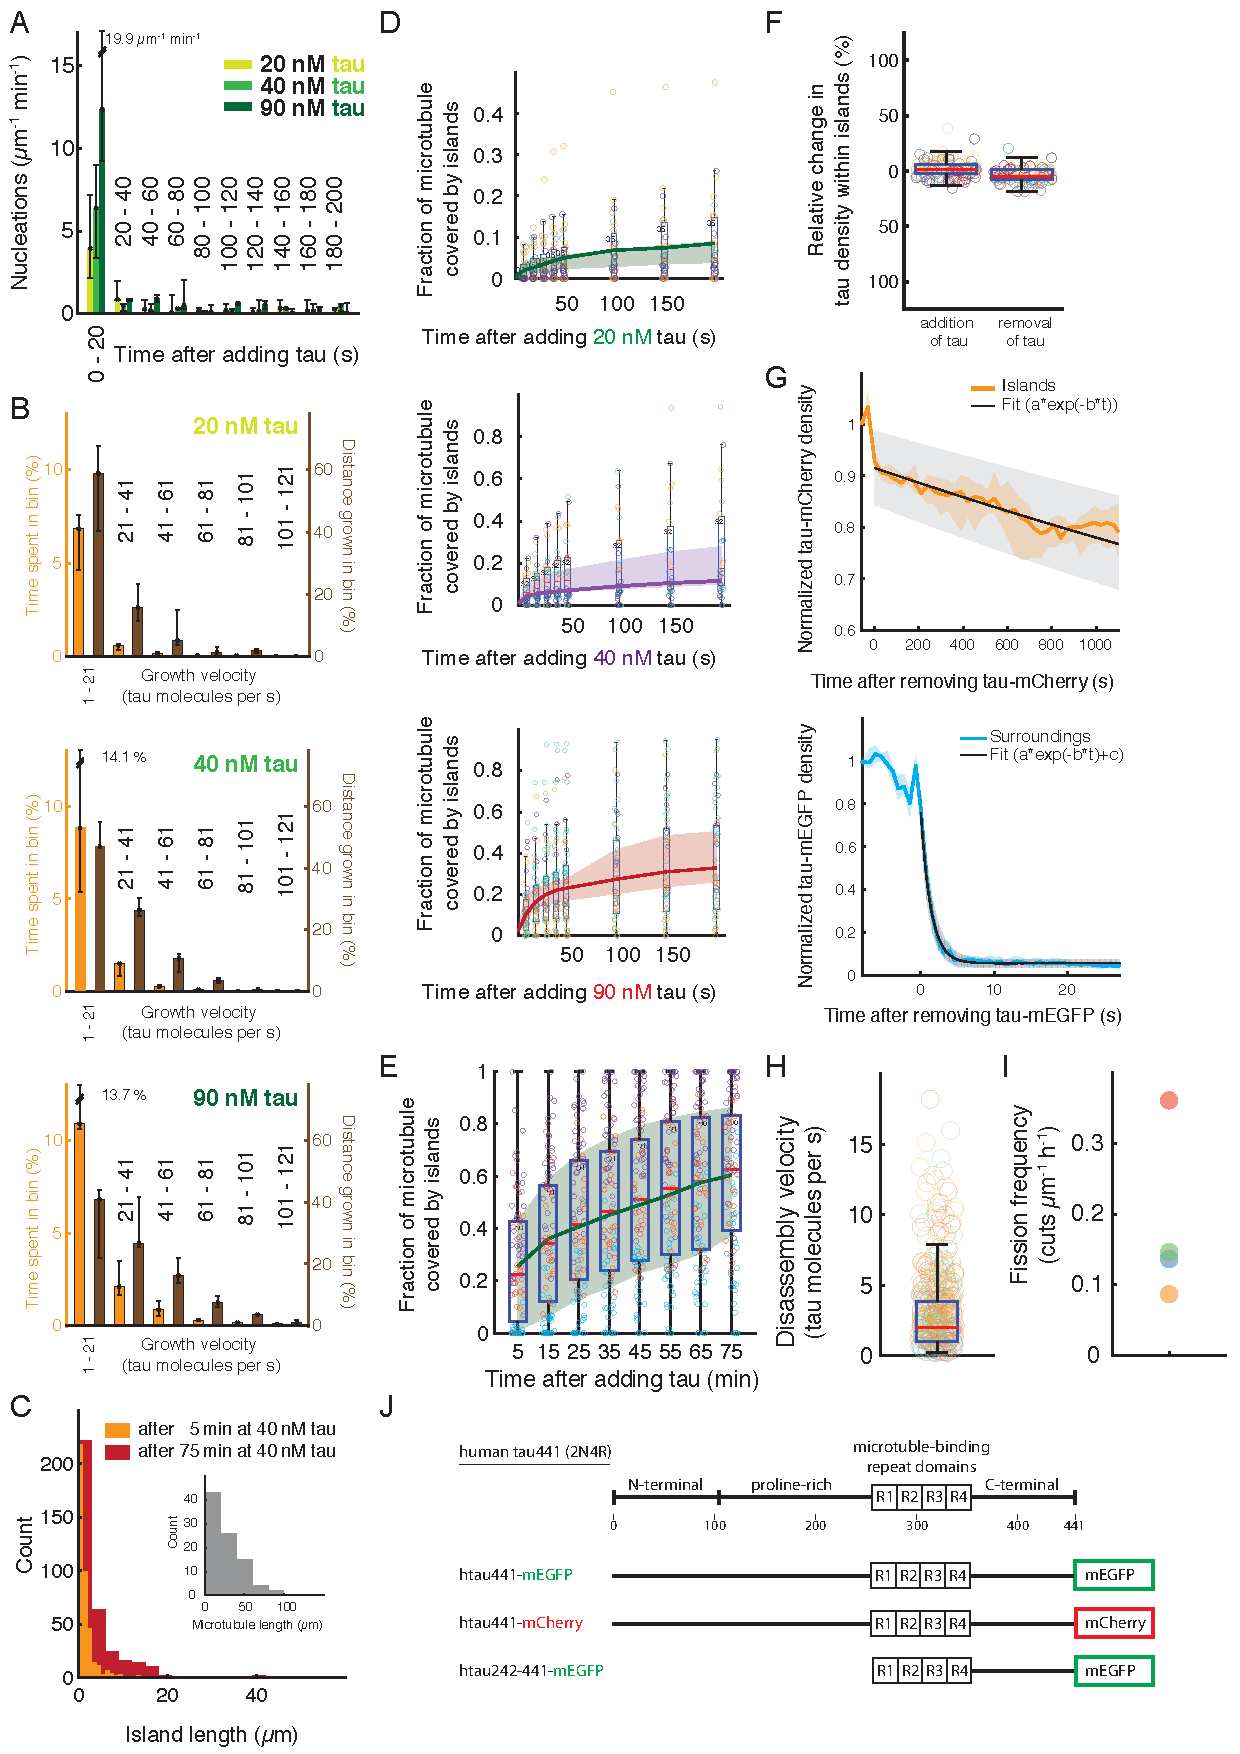
\includegraphics[scale=0.75]{Figures/tau_s1.pdf}
\caption[Supplementary figure for: Tau on microtubules separates into two kinetically distinct phases.]{
Caption on next page.
	}\label{tau_s1}
\end{figure}
\begin{figure}[t]
  \caption{
 (A) Distribution of time between the addition of tau-mEGFP and the formation of the islands (3 experiments per condition, n = 610 nucleation events). Bars show the median; error bars show the minimum and the maximum value. Same experiments as presented in (B) and (D). (B) Histograms of island growth velocities at different tau concentrations in solution (Methods, n = 2131 velocity traces). Same experiments and data representation as in (A). (C) Distribution of the lengths of islands 5 and 75 minutes after the addition of 40 nM tau-mEGFP, n = 91 microtubules in 3 experiments. Distribution of microtubule lengths is shown in the inset. Same experiments as presented in (E). (D) Fraction of microtubule length covered by tau islands at different concentrations of tau-mEGFP in solution. Solid lines and shaded areas (shown also in Figure 1E) represent the median and first and third quartiles values calculated over the whole fields of view (n = 3 experiments). Boxplots represent the same statistics calculated over individual microtubules (n = 40 microtubules for 20 nM tau, n = 32 microtubules for 40 nM tau and n = 59 microtubules for 100 nM tau). The same data as presented in Figure 1E, same experiments as presented in (A). (E) Island assembly does not cease even 75 minutes after the addition of 20 nM tau. The same data representation as in (D), same experiments as presented in (C). (F) Relative difference in tau density within islands i) just after the island nucleation upon the addition of tau and 30 seconds later and ii) just after the removal of tau and 30 seconds later (n = 91 microtubules in 16 experiments). Bleaching was not negligible in the case where tau was absent from solution – for a precise estimation of tau unbinding see (G). (G) Exemplary time-trace of tau-mCherry density inside and tau-mEGFP density outside the islands after removal of tau (mCherry- or mEGFP-labeled, respectively) from solution, analogous to the results presented in Figure 1H (n = 6 microtubules). Single exponential fits are indicated by solid lines. This experiment had been repeated 4 and 3 times for islands and surroundings, respectively, with similar results. Time constants derived from fits for all experiments are shown in Figures 2B and S2D. (H) Distribution of island disassembly velocities upon removal of tau from solution yielding the average velocity of 6.6 ± 5.2 nm/s (average ± SD, corresponding to 2.9 ± 2.3 tau molecules unbinding per second, Methods). Colors encode experiments (n = 335 velocity traces on 90 islands in 4 experiments). For a description of all boxplot elements see Methods. (I) Frequency of fissions occurring within islands upon removal of tau from solution yielding the average 0.20 ± 0.14 fissions per micron of island length per hour (average ± SD). Colors encode n = 4 experiments - same as in (H). (J) Schematics showing the tau constructs used in this study.
  }
\end{figure}
\begin{figure}[h!tb]
\centering
%\includegraphics[scale=0.75]{Figures/tau_s2.png}
\caption[Supplementary figure for: Tau molecules in the islands are stationary but exchange with tau in solution.]{
(A) Exemplary time-trace and fit of tau-mCherry density inside and outside the islands after exchange of 20 nM tau-mCherry for 20 nM tau-mEGFP (n = 5 respectively 7 microtubules). Photo-bleaching during these experiments was negligible (Methods). This experiment had been repeated 5 and 2 times for islands and surroundings, respectively, with similar results. Time constants derived from fits for all experiments are shown in Figures \ref{tau2}C and D. (B) Analogous estimation of tau residence times as in (A) for an exemplary experiment in which 20 nM tau-mCherry was exchanged for 100 nM tau-mEGFP (n = 5 microtubules). The photo-bleaching during this experiment was negligible (Methods). This experiment had been repeated 4 and 2 times for islands and surroundings, respectively, with similar results. Time constants derived from fits for all experiments are shown in Figures \ref{tau2}C and D. (C) Histogram of fluorescence intensities of single tau-mEGFP particles bound to microtubules in experiments as presented in Figure \ref{tau2}E, showing that tau-mEGFP is associated with the microtubule in monomeric form (n = 1861 molecules inside the islands, n = 2210 molecules outside the islands, 1 experiment). (D) Mean square displacement over time of single tau-EGFP molecules inside and outside the islands yielding tau diffusion constants of 0.27 ± 0.15 µm2s-1 (95\% confidence bounds, n = 3660 molecules) outside the islands and 0.027  ± 0.016 µm2s-1 (95\% confidence bounds, n = 2558 molecules, 3 experiments) inside the islands. For comparison, the analogously estimated diffusion constant of non-motile kinesin-1 molecules tightly bound to the microtubule in the presence of AMP-PNP (in the absence of ATP) was 0.014 ± 0.016 µm2s-1 (95\% confidence bounds, n = 126 molecules, 1 experiment).
	}\label{tau_s2}
\end{figure}
\begin{figure}[h!tb]
\centering
%\includegraphics[scale=0.9]{Figures/tau_s4.png}
\caption[Supplementary figure for: Tau islands are distinguished by tau cohesion.]{ (A) Multichannel fluorescence kymograph showing the motion of kip3-GFP (green) inside and outside the tau islands (red). Red arrow indicates the accumulation of kip3-GFP in front of the island. White arrows indicate kip3-GFP molecules speeding up as they leave the island. Scale bar 2 µm. This experiment had been repeated 7 times with similar results. 
	}\label{tau_s4}
\end{figure}
\begin{figure}[h!tb]
\centering
%\includegraphics[scale=0.9]{Figures/tau_s5.png}
\caption[Supplementary figure for: Tau islands are distinguished by tau cohesion.]{
(A) The density of tau-mEGFP on the microtubules saturates at high (µM) tau-mEGFP concentrations (total of 29 and 27 experiments for islands and surroundings, respectively). Horizontal lines indicate the three quartiles. (B) At tau-mEGFP concentrations in the range of 20 nM to approximately 1 µM, the tau-mEGFP density inside the islands scales linearly with the tau-mEGFP density outside the islands. Points indicate medians, error bars indicate the first and third quartiles (both axes). Data from the experiments presented in (A).
	}\label{tau_s5}
\end{figure}

\begin{figure}[h!tb]
\centering
%\includegraphics[scale=0.82]{Figures/tau_s7.png}
\caption[Tau islands do not form at regions of high microtubule curvature.]{
\textbf{Supplementary figure for: Tau islands do not form at regions of high microtubule curvature.} 
(A) Densities of tau-mCherry outside the islands, inside the islands and in the regions of high curvature (after the removal of 0.8 µM tau from solution). Points are color-coded by experiments, horizontal lines indicate the three quartiles, weighted such that each experiment has equal weight. 
(B) Tau density profile along the microtubule after removing 800 nM tau from solution. X-axis is centered on the point of highest curvature. Data are color-coded by microtubule and the density is normalized to the 90th percentile of the density-values of the respective microtubule. The red line represents the median of n = 30 microtubules (7 experiments), the first and third quartile are indicated by the shaded area. At 800 nM tau, there always were islands adjacent to microtubule bends, which is why the tau density to the left and right of the curved microtubule region is high even though tau has been removed from solution. A clear decrease in the tau density is apparent at the point of highest curvature.
(C) Kymograph showing the uniform increase of tau-mEGFP density along the whole region of the microtubule curve upon the addition of tau-mEGFP in solution. This is in strong contrast to islands localized on straight microtubules, which grew at their boundaries. Scale bars, vertical 10 min, horizontal 2 µm.
	}\label{tau_s7}
\end{figure}


\end{document}  